\documentclass[a4paper,pdftex,10pt]{article}
\usepackage[margin=2.5cm,nohead]{geometry}
\usepackage[utf8]{inputenc}
\usepackage[T1]{fontenc} 
\usepackage[english,slovene]{babel} 
\usepackage{amsmath,amsfonts,amsthm,amssymb,mathrsfs,empheq} % Math packages
\usepackage{mathtools}
\usepackage{dsfont}
\usepackage{wrapfig}
\usepackage[pdftex]{graphicx}
%\usepackage{makeidx}
\usepackage{url}
\usepackage{caption}
\usepackage{subcaption}
\usepackage{tabularx}
\usepackage{float}

\usepackage[version=3]{mhchem} %kemija

\DeclarePairedDelimiter{\evdel}{\langle}{\rangle}   %pricakovana vrednost


\renewcommand{\vec}[1]{\boldsymbol{\mathbf{#1}}}                                        
\newcommand{\ihat}[0]{\boldsymbol{\mathbf{\oldhat{\textbf{\i}}}}} % pokončna j in i (j i n i
\newcommand{\iu}{{i\mkern1mu}}	    %imaginarno število
\DeclarePairedDelimiterX{\norm}[1]{\lVert}{\rVert}{#1} %norma

\usepackage{fancyhdr} % Custom headers and footers
\pagestyle{fancyplain} % Makes all pages in the document conform to the custom headers and footers
\fancyhead{} % No page header - if you want one, create it in the same way as the footers below
\fancyfoot[L]{} % Empty left footer
\fancyfoot[C]{} % Empty center footer
\fancyfoot[R]{\thepage} % Page numbering for right footer
\renewcommand{\headrulewidth}{0pt} % Remove header underlines
\renewcommand{\footrulewidth}{0pt} % Remove footer underlines
\setlength{\headheight}{13.6pt} % Customize the height of the header

%\numberwithin{equation}{section} % Number equations within sections (i.e. 1.1, 1.2, 2.1, 2.2 instead of 1, 2, 3, 4)
\numberwithin{figure}{section} % Number figures within sections (i.e. 1.1, 1.2, 2.1, 2.2 instead of 1, 2, 3, 4)
%\numberwithin{table}{section} % Number tables within sections (i.e. 1.1, 1.2, 2.1, 2.2 instead of 1, 2, 3, 4)

\setlength\parindent{0pt} % Removes all indentation from paragraphs - comment this line for an assignment with lots of text

%----------------------------------------------------------------------------------------
%	TITLE SECTION
%----------------------------------------------------------------------------------------

\newcommand{\horrule}[1]{\rule{\linewidth}{#1}} % Create horizontal rule command with 1 argument of height

\title{	
\normalfont \normalsize 
\textsc{Modelska analiza 1} \\ [25pt] % Your university, school and/or department name(s)
%\horrule{0.2pt} \\[0.4cm] % Thin top horizontal rule
\huge 10. naloga - Spektralna analiza in filtriranje\\ % The assignment title
%\horrule{0.2pt} \\[0.5cm] % Thick bottom horizontal rule
}

\author{Tina Klobas} % Your name

\date{\normalsize\today} % Today's date or a custom date

\begin{document}

\maketitle % Print the title

\section{Opis problema}
Pri tej nalogi si bomo pogledali tri različne primere spektralne analize in filtriranja
podatkov. Z~diskretno Fourierovo transformacijo:
\begin{equation}
    F_k = \frac{1}{N} \sum_{j=0}^{N-1} f_j \mathrm{e}^{- 2\pi \mathrm{i} j k /N},
\end{equation}
vhodnega signala dobimo frekvenčni spekter, s~čimer dobimo informacijo o~fazah in amplitudah
signala. Moč spektra izračunamo kot:
\begin{equation}
    P_k = \frac{1}{2} ( | F_k |^2 + |F_{N-k}|^2 ). 
\end{equation}
V~prvem delu si bomo pogledali, kako razpon podatkov in izbira okenskih funkcij vpliva
na dobljen spekter. V~naslednjem odseku rekonstruirali vpadne signale iz dobljenih signalov,
iz katerih bomo z~Wienerjevim filtrom odstranili šum. Na koncu si bomo pogledali še 
rekonstrukcijo zašumljenih slik.

%----------------------------------------------------------------------------------------
%	PROBLEM 1
%----------------------------------------------------------------------------------------
\section{Določanje frekvenčnega spektra}
V~datotekah \path{val2.dat} in \path{val3.dat} imamo shranjena signala s~$512$ točkami in
jima želimo določiti frekvenčni spekter. Izhodni signal, je prikazan na grafu~\ref{slika1}. 
\begin{figure}[H] 
    \centering
    \resizebox{0.49\linewidth}{!}{% GNUPLOT: LaTeX picture with Postscript
\begingroup
  \makeatletter
  \providecommand\color[2][]{%
    \GenericError{(gnuplot) \space\space\space\@spaces}{%
      Package color not loaded in conjunction with
      terminal option `colourtext'%
    }{See the gnuplot documentation for explanation.%
    }{Either use 'blacktext' in gnuplot or load the package
      color.sty in LaTeX.}%
    \renewcommand\color[2][]{}%
  }%
  \providecommand\includegraphics[2][]{%
    \GenericError{(gnuplot) \space\space\space\@spaces}{%
      Package graphicx or graphics not loaded%
    }{See the gnuplot documentation for explanation.%
    }{The gnuplot epslatex terminal needs graphicx.sty or graphics.sty.}%
    \renewcommand\includegraphics[2][]{}%
  }%
  \providecommand\rotatebox[2]{#2}%
  \@ifundefined{ifGPcolor}{%
    \newif\ifGPcolor
    \GPcolortrue
  }{}%
  \@ifundefined{ifGPblacktext}{%
    \newif\ifGPblacktext
    \GPblacktexttrue
  }{}%
  % define a \g@addto@macro without @ in the name:
  \let\gplgaddtomacro\g@addto@macro
  % define empty templates for all commands taking text:
  \gdef\gplbacktext{}%
  \gdef\gplfronttext{}%
  \makeatother
  \ifGPblacktext
    % no textcolor at all
    \def\colorrgb#1{}%
    \def\colorgray#1{}%
  \else
    % gray or color?
    \ifGPcolor
      \def\colorrgb#1{\color[rgb]{#1}}%
      \def\colorgray#1{\color[gray]{#1}}%
      \expandafter\def\csname LTw\endcsname{\color{white}}%
      \expandafter\def\csname LTb\endcsname{\color{black}}%
      \expandafter\def\csname LTa\endcsname{\color{black}}%
      \expandafter\def\csname LT0\endcsname{\color[rgb]{1,0,0}}%
      \expandafter\def\csname LT1\endcsname{\color[rgb]{0,1,0}}%
      \expandafter\def\csname LT2\endcsname{\color[rgb]{0,0,1}}%
      \expandafter\def\csname LT3\endcsname{\color[rgb]{1,0,1}}%
      \expandafter\def\csname LT4\endcsname{\color[rgb]{0,1,1}}%
      \expandafter\def\csname LT5\endcsname{\color[rgb]{1,1,0}}%
      \expandafter\def\csname LT6\endcsname{\color[rgb]{0,0,0}}%
      \expandafter\def\csname LT7\endcsname{\color[rgb]{1,0.3,0}}%
      \expandafter\def\csname LT8\endcsname{\color[rgb]{0.5,0.5,0.5}}%
    \else
      % gray
      \def\colorrgb#1{\color{black}}%
      \def\colorgray#1{\color[gray]{#1}}%
      \expandafter\def\csname LTw\endcsname{\color{white}}%
      \expandafter\def\csname LTb\endcsname{\color{black}}%
      \expandafter\def\csname LTa\endcsname{\color{black}}%
      \expandafter\def\csname LT0\endcsname{\color{black}}%
      \expandafter\def\csname LT1\endcsname{\color{black}}%
      \expandafter\def\csname LT2\endcsname{\color{black}}%
      \expandafter\def\csname LT3\endcsname{\color{black}}%
      \expandafter\def\csname LT4\endcsname{\color{black}}%
      \expandafter\def\csname LT5\endcsname{\color{black}}%
      \expandafter\def\csname LT6\endcsname{\color{black}}%
      \expandafter\def\csname LT7\endcsname{\color{black}}%
      \expandafter\def\csname LT8\endcsname{\color{black}}%
    \fi
  \fi
    \setlength{\unitlength}{0.0500bp}%
    \ifx\gptboxheight\undefined%
      \newlength{\gptboxheight}%
      \newlength{\gptboxwidth}%
      \newsavebox{\gptboxtext}%
    \fi%
    \setlength{\fboxrule}{0.5pt}%
    \setlength{\fboxsep}{1pt}%
\begin{picture}(7180.00,4300.00)%
    \gplgaddtomacro\gplbacktext{%
      \csname LTb\endcsname%%
      \put(932,652){\makebox(0,0)[r]{\strut{}$-4000$}}%
      \csname LTb\endcsname%%
      \put(932,1800){\makebox(0,0)[r]{\strut{}$0$}}%
      \csname LTb\endcsname%%
      \put(932,2947){\makebox(0,0)[r]{\strut{}$4000$}}%
      \csname LTb\endcsname%%
      \put(932,4095){\makebox(0,0)[r]{\strut{}$8000$}}%
      \csname LTb\endcsname%%
      \put(1872,448){\makebox(0,0){\strut{}$0$}}%
      \csname LTb\endcsname%%
      \put(3529,448){\makebox(0,0){\strut{}$10000$}}%
      \csname LTb\endcsname%%
      \put(5186,448){\makebox(0,0){\strut{}$20000$}}%
      \csname LTb\endcsname%%
      \put(6843,448){\makebox(0,0){\strut{}$30000$}}%
    }%
    \gplgaddtomacro\gplfronttext{%
      \csname LTb\endcsname%%
      \put(186,2373){\rotatebox{-270}{\makebox(0,0){\strut{}$y(t)$}}}%
      \csname LTb\endcsname%%
      \put(3943,142){\makebox(0,0){\strut{}$x(t)$}}%
      \csname LTb\endcsname%%
      \put(1573,3688){\makebox(0,0)[l]{\strut{}Kontrola}}%
      \csname LTb\endcsname%%
      \put(1573,3892){\makebox(0,0)[l]{\strut{}Kalman}}%
    }%
    \gplbacktext
    \put(0,0){\includegraphics{graf1a}}%
    \gplfronttext
  \end{picture}%
\endgroup
}
    \resizebox{0.49\linewidth}{!}{% GNUPLOT: LaTeX picture with Postscript
\begingroup
  \makeatletter
  \providecommand\color[2][]{%
    \GenericError{(gnuplot) \space\space\space\@spaces}{%
      Package color not loaded in conjunction with
      terminal option `colourtext'%
    }{See the gnuplot documentation for explanation.%
    }{Either use 'blacktext' in gnuplot or load the package
      color.sty in LaTeX.}%
    \renewcommand\color[2][]{}%
  }%
  \providecommand\includegraphics[2][]{%
    \GenericError{(gnuplot) \space\space\space\@spaces}{%
      Package graphicx or graphics not loaded%
    }{See the gnuplot documentation for explanation.%
    }{The gnuplot epslatex terminal needs graphicx.sty or graphics.sty.}%
    \renewcommand\includegraphics[2][]{}%
  }%
  \providecommand\rotatebox[2]{#2}%
  \@ifundefined{ifGPcolor}{%
    \newif\ifGPcolor
    \GPcolortrue
  }{}%
  \@ifundefined{ifGPblacktext}{%
    \newif\ifGPblacktext
    \GPblacktexttrue
  }{}%
  % define a \g@addto@macro without @ in the name:
  \let\gplgaddtomacro\g@addto@macro
  % define empty templates for all commands taking text:
  \gdef\gplbacktext{}%
  \gdef\gplfronttext{}%
  \makeatother
  \ifGPblacktext
    % no textcolor at all
    \def\colorrgb#1{}%
    \def\colorgray#1{}%
  \else
    % gray or color?
    \ifGPcolor
      \def\colorrgb#1{\color[rgb]{#1}}%
      \def\colorgray#1{\color[gray]{#1}}%
      \expandafter\def\csname LTw\endcsname{\color{white}}%
      \expandafter\def\csname LTb\endcsname{\color{black}}%
      \expandafter\def\csname LTa\endcsname{\color{black}}%
      \expandafter\def\csname LT0\endcsname{\color[rgb]{1,0,0}}%
      \expandafter\def\csname LT1\endcsname{\color[rgb]{0,1,0}}%
      \expandafter\def\csname LT2\endcsname{\color[rgb]{0,0,1}}%
      \expandafter\def\csname LT3\endcsname{\color[rgb]{1,0,1}}%
      \expandafter\def\csname LT4\endcsname{\color[rgb]{0,1,1}}%
      \expandafter\def\csname LT5\endcsname{\color[rgb]{1,1,0}}%
      \expandafter\def\csname LT6\endcsname{\color[rgb]{0,0,0}}%
      \expandafter\def\csname LT7\endcsname{\color[rgb]{1,0.3,0}}%
      \expandafter\def\csname LT8\endcsname{\color[rgb]{0.5,0.5,0.5}}%
    \else
      % gray
      \def\colorrgb#1{\color{black}}%
      \def\colorgray#1{\color[gray]{#1}}%
      \expandafter\def\csname LTw\endcsname{\color{white}}%
      \expandafter\def\csname LTb\endcsname{\color{black}}%
      \expandafter\def\csname LTa\endcsname{\color{black}}%
      \expandafter\def\csname LT0\endcsname{\color{black}}%
      \expandafter\def\csname LT1\endcsname{\color{black}}%
      \expandafter\def\csname LT2\endcsname{\color{black}}%
      \expandafter\def\csname LT3\endcsname{\color{black}}%
      \expandafter\def\csname LT4\endcsname{\color{black}}%
      \expandafter\def\csname LT5\endcsname{\color{black}}%
      \expandafter\def\csname LT6\endcsname{\color{black}}%
      \expandafter\def\csname LT7\endcsname{\color{black}}%
      \expandafter\def\csname LT8\endcsname{\color{black}}%
    \fi
  \fi
    \setlength{\unitlength}{0.0500bp}%
    \ifx\gptboxheight\undefined%
      \newlength{\gptboxheight}%
      \newlength{\gptboxwidth}%
      \newsavebox{\gptboxtext}%
    \fi%
    \setlength{\fboxrule}{0.5pt}%
    \setlength{\fboxsep}{1pt}%
\begin{picture}(7200.00,5040.00)%
    \gplgaddtomacro\gplbacktext{%
      \csname LTb\endcsname%%
      \put(682,704){\makebox(0,0)[r]{\strut{}$-8$}}%
      \put(682,1218){\makebox(0,0)[r]{\strut{}$-6$}}%
      \put(682,1733){\makebox(0,0)[r]{\strut{}$-4$}}%
      \put(682,2247){\makebox(0,0)[r]{\strut{}$-2$}}%
      \put(682,2762){\makebox(0,0)[r]{\strut{}$0$}}%
      \put(682,3276){\makebox(0,0)[r]{\strut{}$2$}}%
      \put(682,3790){\makebox(0,0)[r]{\strut{}$4$}}%
      \put(682,4305){\makebox(0,0)[r]{\strut{}$6$}}%
      \put(682,4819){\makebox(0,0)[r]{\strut{}$8$}}%
      \put(814,484){\makebox(0,0){\strut{}$0$}}%
      \put(2012,484){\makebox(0,0){\strut{}$0.2$}}%
      \put(3210,484){\makebox(0,0){\strut{}$0.4$}}%
      \put(4407,484){\makebox(0,0){\strut{}$0.6$}}%
      \put(5605,484){\makebox(0,0){\strut{}$0.8$}}%
      \put(6803,484){\makebox(0,0){\strut{}$1$}}%
    }%
    \gplgaddtomacro\gplfronttext{%
      \csname LTb\endcsname%%
      \put(209,2761){\rotatebox{-270}{\makebox(0,0){\strut{}$f(t)$}}}%
      \put(3808,154){\makebox(0,0){\strut{}$t$}}%
    }%
    \gplbacktext
    \put(0,0){\includegraphics[width={360.00bp},height={252.00bp}]{graf1b}}%
    \gplfronttext
  \end{picture}%
\endgroup
}
    \caption{Vhodna signala -- na levi \protect\path{val2.dat} in na desni 
    \protect\path{val3.dat}.}
    \label{slika1}
\end{figure}

\subsection{Reševanje in rezultati}
Na sliki~\ref{slika2} sta prikazana spektra moči signalov v~logaritemski skali.
\begin{figure}[H]
    \centering
    \resizebox{0.8\linewidth}{!}{% GNUPLOT: LaTeX picture with Postscript
\begingroup
  \makeatletter
  \providecommand\color[2][]{%
    \GenericError{(gnuplot) \space\space\space\@spaces}{%
      Package color not loaded in conjunction with
      terminal option `colourtext'%
    }{See the gnuplot documentation for explanation.%
    }{Either use 'blacktext' in gnuplot or load the package
      color.sty in LaTeX.}%
    \renewcommand\color[2][]{}%
  }%
  \providecommand\includegraphics[2][]{%
    \GenericError{(gnuplot) \space\space\space\@spaces}{%
      Package graphicx or graphics not loaded%
    }{See the gnuplot documentation for explanation.%
    }{The gnuplot epslatex terminal needs graphicx.sty or graphics.sty.}%
    \renewcommand\includegraphics[2][]{}%
  }%
  \providecommand\rotatebox[2]{#2}%
  \@ifundefined{ifGPcolor}{%
    \newif\ifGPcolor
    \GPcolortrue
  }{}%
  \@ifundefined{ifGPblacktext}{%
    \newif\ifGPblacktext
    \GPblacktexttrue
  }{}%
  % define a \g@addto@macro without @ in the name:
  \let\gplgaddtomacro\g@addto@macro
  % define empty templates for all commands taking text:
  \gdef\gplbacktext{}%
  \gdef\gplfronttext{}%
  \makeatother
  \ifGPblacktext
    % no textcolor at all
    \def\colorrgb#1{}%
    \def\colorgray#1{}%
  \else
    % gray or color?
    \ifGPcolor
      \def\colorrgb#1{\color[rgb]{#1}}%
      \def\colorgray#1{\color[gray]{#1}}%
      \expandafter\def\csname LTw\endcsname{\color{white}}%
      \expandafter\def\csname LTb\endcsname{\color{black}}%
      \expandafter\def\csname LTa\endcsname{\color{black}}%
      \expandafter\def\csname LT0\endcsname{\color[rgb]{1,0,0}}%
      \expandafter\def\csname LT1\endcsname{\color[rgb]{0,1,0}}%
      \expandafter\def\csname LT2\endcsname{\color[rgb]{0,0,1}}%
      \expandafter\def\csname LT3\endcsname{\color[rgb]{1,0,1}}%
      \expandafter\def\csname LT4\endcsname{\color[rgb]{0,1,1}}%
      \expandafter\def\csname LT5\endcsname{\color[rgb]{1,1,0}}%
      \expandafter\def\csname LT6\endcsname{\color[rgb]{0,0,0}}%
      \expandafter\def\csname LT7\endcsname{\color[rgb]{1,0.3,0}}%
      \expandafter\def\csname LT8\endcsname{\color[rgb]{0.5,0.5,0.5}}%
    \else
      % gray
      \def\colorrgb#1{\color{black}}%
      \def\colorgray#1{\color[gray]{#1}}%
      \expandafter\def\csname LTw\endcsname{\color{white}}%
      \expandafter\def\csname LTb\endcsname{\color{black}}%
      \expandafter\def\csname LTa\endcsname{\color{black}}%
      \expandafter\def\csname LT0\endcsname{\color{black}}%
      \expandafter\def\csname LT1\endcsname{\color{black}}%
      \expandafter\def\csname LT2\endcsname{\color{black}}%
      \expandafter\def\csname LT3\endcsname{\color{black}}%
      \expandafter\def\csname LT4\endcsname{\color{black}}%
      \expandafter\def\csname LT5\endcsname{\color{black}}%
      \expandafter\def\csname LT6\endcsname{\color{black}}%
      \expandafter\def\csname LT7\endcsname{\color{black}}%
      \expandafter\def\csname LT8\endcsname{\color{black}}%
    \fi
  \fi
    \setlength{\unitlength}{0.0500bp}%
    \ifx\gptboxheight\undefined%
      \newlength{\gptboxheight}%
      \newlength{\gptboxwidth}%
      \newsavebox{\gptboxtext}%
    \fi%
    \setlength{\fboxrule}{0.5pt}%
    \setlength{\fboxsep}{1pt}%
\begin{picture}(7200.00,5040.00)%
    \gplgaddtomacro\gplbacktext{%
      \csname LTb\endcsname%%
      \put(946,2350){\makebox(0,0)[r]{\strut{}$1$}}%
      \put(946,704){\makebox(0,0)[r]{\strut{}$10^{-4}$}}%
      \put(946,1527){\makebox(0,0)[r]{\strut{}$10^{-2}$}}%
      \put(946,3173){\makebox(0,0)[r]{\strut{}$10^{2}$}}%
      \put(946,3996){\makebox(0,0)[r]{\strut{}$10^{4}$}}%
      \put(946,4819){\makebox(0,0)[r]{\strut{}$10^{6}$}}%
      \put(1078,484){\makebox(0,0){\strut{}$0$}}%
      \put(2223,484){\makebox(0,0){\strut{}$0.1$}}%
      \put(3368,484){\makebox(0,0){\strut{}$0.2$}}%
      \put(4513,484){\makebox(0,0){\strut{}$0.3$}}%
      \put(5658,484){\makebox(0,0){\strut{}$0.4$}}%
      \put(6803,484){\makebox(0,0){\strut{}$0.5$}}%
    }%
    \gplgaddtomacro\gplfronttext{%
      \csname LTb\endcsname%%
      \put(209,2761){\rotatebox{-270}{\makebox(0,0){\strut{}$|f|^2$}}}%
      \put(3940,154){\makebox(0,0){\strut{}$\omega$}}%
      \csname LTb\endcsname%%
      \put(1669,4404){\makebox(0,0)[l]{\strut{}val2}}%
      \csname LTb\endcsname%%
      \put(1669,4624){\makebox(0,0)[l]{\strut{}val3}}%
    }%
    \gplbacktext
    \put(0,0){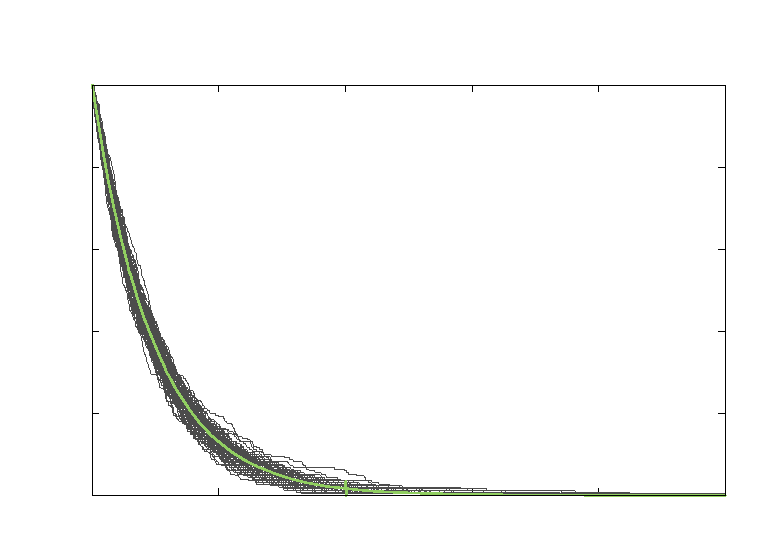
\includegraphics[width={360.00bp},height={252.00bp}]{graf2}}%
    \gplfronttext
  \end{picture}%
\endgroup
}
    \caption{Spektra signalov v~logaritemski skali.}
    \label{slika2}
\end{figure}
Fourierova transformacija deluje dobro za periodične funkcije -- v~našem primeru vidimo, da
ima dobljen graf za prvi spekter -- \emph{val2} -- dva izrazita vrha, kar kaže na 
periodičnost spektra, medtem ko so vsi štirje vrhovi drugega spektra -- \emph{val3} -- 
precej razširjeni, kar opozarja na nasprotno. \\
Najprej lahko preverimo, kaj se zgodi, če vzamemo krajše intervale točk; ${62,128,256}$. 
Naslednji graf~\ref{slika3} prikazuje spektre izračunane za štiri različne intervale točk. 
Za prvi spekter vidimo, da ima bolj ali manj enako obliko in širino vrhov -- razen za 
interval z~$64$ točkami, ki je bil očitno prekratek in smo izgubili informacije o~spektru. 
Za drugi spekter, pa vidimo, da se vrhovi zelo razširijo in spremenijo obliko -- sumimo, 
da že v~začetku nismo ujeli periodičnosti signala.\\
\begin{figure}[H]
    \centering
    \resizebox{0.49\linewidth}{!}{% GNUPLOT: LaTeX picture with Postscript
\begingroup
  \makeatletter
  \providecommand\color[2][]{%
    \GenericError{(gnuplot) \space\space\space\@spaces}{%
      Package color not loaded in conjunction with
      terminal option `colourtext'%
    }{See the gnuplot documentation for explanation.%
    }{Either use 'blacktext' in gnuplot or load the package
      color.sty in LaTeX.}%
    \renewcommand\color[2][]{}%
  }%
  \providecommand\includegraphics[2][]{%
    \GenericError{(gnuplot) \space\space\space\@spaces}{%
      Package graphicx or graphics not loaded%
    }{See the gnuplot documentation for explanation.%
    }{The gnuplot epslatex terminal needs graphicx.sty or graphics.sty.}%
    \renewcommand\includegraphics[2][]{}%
  }%
  \providecommand\rotatebox[2]{#2}%
  \@ifundefined{ifGPcolor}{%
    \newif\ifGPcolor
    \GPcolortrue
  }{}%
  \@ifundefined{ifGPblacktext}{%
    \newif\ifGPblacktext
    \GPblacktexttrue
  }{}%
  % define a \g@addto@macro without @ in the name:
  \let\gplgaddtomacro\g@addto@macro
  % define empty templates for all commands taking text:
  \gdef\gplbacktext{}%
  \gdef\gplfronttext{}%
  \makeatother
  \ifGPblacktext
    % no textcolor at all
    \def\colorrgb#1{}%
    \def\colorgray#1{}%
  \else
    % gray or color?
    \ifGPcolor
      \def\colorrgb#1{\color[rgb]{#1}}%
      \def\colorgray#1{\color[gray]{#1}}%
      \expandafter\def\csname LTw\endcsname{\color{white}}%
      \expandafter\def\csname LTb\endcsname{\color{black}}%
      \expandafter\def\csname LTa\endcsname{\color{black}}%
      \expandafter\def\csname LT0\endcsname{\color[rgb]{1,0,0}}%
      \expandafter\def\csname LT1\endcsname{\color[rgb]{0,1,0}}%
      \expandafter\def\csname LT2\endcsname{\color[rgb]{0,0,1}}%
      \expandafter\def\csname LT3\endcsname{\color[rgb]{1,0,1}}%
      \expandafter\def\csname LT4\endcsname{\color[rgb]{0,1,1}}%
      \expandafter\def\csname LT5\endcsname{\color[rgb]{1,1,0}}%
      \expandafter\def\csname LT6\endcsname{\color[rgb]{0,0,0}}%
      \expandafter\def\csname LT7\endcsname{\color[rgb]{1,0.3,0}}%
      \expandafter\def\csname LT8\endcsname{\color[rgb]{0.5,0.5,0.5}}%
    \else
      % gray
      \def\colorrgb#1{\color{black}}%
      \def\colorgray#1{\color[gray]{#1}}%
      \expandafter\def\csname LTw\endcsname{\color{white}}%
      \expandafter\def\csname LTb\endcsname{\color{black}}%
      \expandafter\def\csname LTa\endcsname{\color{black}}%
      \expandafter\def\csname LT0\endcsname{\color{black}}%
      \expandafter\def\csname LT1\endcsname{\color{black}}%
      \expandafter\def\csname LT2\endcsname{\color{black}}%
      \expandafter\def\csname LT3\endcsname{\color{black}}%
      \expandafter\def\csname LT4\endcsname{\color{black}}%
      \expandafter\def\csname LT5\endcsname{\color{black}}%
      \expandafter\def\csname LT6\endcsname{\color{black}}%
      \expandafter\def\csname LT7\endcsname{\color{black}}%
      \expandafter\def\csname LT8\endcsname{\color{black}}%
    \fi
  \fi
    \setlength{\unitlength}{0.0500bp}%
    \ifx\gptboxheight\undefined%
      \newlength{\gptboxheight}%
      \newlength{\gptboxwidth}%
      \newsavebox{\gptboxtext}%
    \fi%
    \setlength{\fboxrule}{0.5pt}%
    \setlength{\fboxsep}{1pt}%
\begin{picture}(7200.00,5040.00)%
    \gplgaddtomacro\gplbacktext{%
      \csname LTb\endcsname%%
      \put(814,704){\makebox(0,0)[r]{\strut{}$-50$}}%
      \put(814,1733){\makebox(0,0)[r]{\strut{}$-25$}}%
      \put(814,2762){\makebox(0,0)[r]{\strut{}$0$}}%
      \put(814,3790){\makebox(0,0)[r]{\strut{}$25$}}%
      \put(814,4819){\makebox(0,0)[r]{\strut{}$50$}}%
      \put(946,484){\makebox(0,0){\strut{}$0$}}%
      \put(2117,484){\makebox(0,0){\strut{}$500$}}%
      \put(3289,484){\makebox(0,0){\strut{}$1000$}}%
      \put(4460,484){\makebox(0,0){\strut{}$1500$}}%
      \put(5632,484){\makebox(0,0){\strut{}$2000$}}%
      \put(6803,484){\makebox(0,0){\strut{}$2500$}}%
    }%
    \gplgaddtomacro\gplfronttext{%
      \csname LTb\endcsname%%
      \put(209,2761){\rotatebox{-270}{\makebox(0,0){\strut{}$x^+ - \hat{x}$}}}%
      \put(3874,154){\makebox(0,0){\strut{}$t$}}%
      \csname LTb\endcsname%%
      \put(1537,3964){\makebox(0,0)[l]{\strut{}$90\%$}}%
      \csname LTb\endcsname%%
      \put(1537,4184){\makebox(0,0)[l]{\strut{}$95\%$}}%
      \csname LTb\endcsname%%
      \put(1537,4404){\makebox(0,0)[l]{\strut{}$99\%$}}%
      \csname LTb\endcsname%%
      \put(1537,4624){\makebox(0,0)[l]{\strut{}$x^+-\hat{x}$}}%
    }%
    \gplbacktext
    \put(0,0){\includegraphics{graf3a}}%
    \gplfronttext
  \end{picture}%
\endgroup
}
    \resizebox{0.49\linewidth}{!}{% GNUPLOT: LaTeX picture with Postscript
\begingroup
  \makeatletter
  \providecommand\color[2][]{%
    \GenericError{(gnuplot) \space\space\space\@spaces}{%
      Package color not loaded in conjunction with
      terminal option `colourtext'%
    }{See the gnuplot documentation for explanation.%
    }{Either use 'blacktext' in gnuplot or load the package
      color.sty in LaTeX.}%
    \renewcommand\color[2][]{}%
  }%
  \providecommand\includegraphics[2][]{%
    \GenericError{(gnuplot) \space\space\space\@spaces}{%
      Package graphicx or graphics not loaded%
    }{See the gnuplot documentation for explanation.%
    }{The gnuplot epslatex terminal needs graphicx.sty or graphics.sty.}%
    \renewcommand\includegraphics[2][]{}%
  }%
  \providecommand\rotatebox[2]{#2}%
  \@ifundefined{ifGPcolor}{%
    \newif\ifGPcolor
    \GPcolortrue
  }{}%
  \@ifundefined{ifGPblacktext}{%
    \newif\ifGPblacktext
    \GPblacktexttrue
  }{}%
  % define a \g@addto@macro without @ in the name:
  \let\gplgaddtomacro\g@addto@macro
  % define empty templates for all commands taking text:
  \gdef\gplbacktext{}%
  \gdef\gplfronttext{}%
  \makeatother
  \ifGPblacktext
    % no textcolor at all
    \def\colorrgb#1{}%
    \def\colorgray#1{}%
  \else
    % gray or color?
    \ifGPcolor
      \def\colorrgb#1{\color[rgb]{#1}}%
      \def\colorgray#1{\color[gray]{#1}}%
      \expandafter\def\csname LTw\endcsname{\color{white}}%
      \expandafter\def\csname LTb\endcsname{\color{black}}%
      \expandafter\def\csname LTa\endcsname{\color{black}}%
      \expandafter\def\csname LT0\endcsname{\color[rgb]{1,0,0}}%
      \expandafter\def\csname LT1\endcsname{\color[rgb]{0,1,0}}%
      \expandafter\def\csname LT2\endcsname{\color[rgb]{0,0,1}}%
      \expandafter\def\csname LT3\endcsname{\color[rgb]{1,0,1}}%
      \expandafter\def\csname LT4\endcsname{\color[rgb]{0,1,1}}%
      \expandafter\def\csname LT5\endcsname{\color[rgb]{1,1,0}}%
      \expandafter\def\csname LT6\endcsname{\color[rgb]{0,0,0}}%
      \expandafter\def\csname LT7\endcsname{\color[rgb]{1,0.3,0}}%
      \expandafter\def\csname LT8\endcsname{\color[rgb]{0.5,0.5,0.5}}%
    \else
      % gray
      \def\colorrgb#1{\color{black}}%
      \def\colorgray#1{\color[gray]{#1}}%
      \expandafter\def\csname LTw\endcsname{\color{white}}%
      \expandafter\def\csname LTb\endcsname{\color{black}}%
      \expandafter\def\csname LTa\endcsname{\color{black}}%
      \expandafter\def\csname LT0\endcsname{\color{black}}%
      \expandafter\def\csname LT1\endcsname{\color{black}}%
      \expandafter\def\csname LT2\endcsname{\color{black}}%
      \expandafter\def\csname LT3\endcsname{\color{black}}%
      \expandafter\def\csname LT4\endcsname{\color{black}}%
      \expandafter\def\csname LT5\endcsname{\color{black}}%
      \expandafter\def\csname LT6\endcsname{\color{black}}%
      \expandafter\def\csname LT7\endcsname{\color{black}}%
      \expandafter\def\csname LT8\endcsname{\color{black}}%
    \fi
  \fi
    \setlength{\unitlength}{0.0500bp}%
    \ifx\gptboxheight\undefined%
      \newlength{\gptboxheight}%
      \newlength{\gptboxwidth}%
      \newsavebox{\gptboxtext}%
    \fi%
    \setlength{\fboxrule}{0.5pt}%
    \setlength{\fboxsep}{1pt}%
\begin{picture}(7200.00,5040.00)%
    \gplgaddtomacro\gplbacktext{%
      \csname LTb\endcsname%%
      \put(946,704){\makebox(0,0)[r]{\strut{}$-100$}}%
      \put(946,1733){\makebox(0,0)[r]{\strut{}$-50$}}%
      \put(946,2762){\makebox(0,0)[r]{\strut{}$0$}}%
      \put(946,3790){\makebox(0,0)[r]{\strut{}$50$}}%
      \put(946,4819){\makebox(0,0)[r]{\strut{}$100$}}%
      \put(1078,484){\makebox(0,0){\strut{}$0$}}%
      \put(2223,484){\makebox(0,0){\strut{}$500$}}%
      \put(3368,484){\makebox(0,0){\strut{}$1000$}}%
      \put(4513,484){\makebox(0,0){\strut{}$1500$}}%
      \put(5658,484){\makebox(0,0){\strut{}$2000$}}%
      \put(6803,484){\makebox(0,0){\strut{}$2500$}}%
    }%
    \gplgaddtomacro\gplfronttext{%
      \csname LTb\endcsname%%
      \put(209,2761){\rotatebox{-270}{\makebox(0,0){\strut{}$x^+ - \hat{x}$}}}%
      \put(3940,154){\makebox(0,0){\strut{}$t$}}%
      \csname LTb\endcsname%%
      \put(1669,3964){\makebox(0,0)[l]{\strut{}$90\%$}}%
      \csname LTb\endcsname%%
      \put(1669,4184){\makebox(0,0)[l]{\strut{}$95\%$}}%
      \csname LTb\endcsname%%
      \put(1669,4404){\makebox(0,0)[l]{\strut{}$99\%$}}%
      \csname LTb\endcsname%%
      \put(1669,4624){\makebox(0,0)[l]{\strut{}$x^+-\hat{x}$}}%
    }%
    \gplbacktext
    \put(0,0){\includegraphics{graf3b}}%
    \gplfronttext
  \end{picture}%
\endgroup
}
    \caption{Spektri moči (na levi \protect\path{val2} in na desni \protect\path{val3} za 
    različne intervale.}
    \label{slika3}
\end{figure}
Poskusimo obdelati signal še z~različnimi okenskimi funkcijami, ki signal na robu postavijo
na nič -- da dobimo periodičnost signala:
\begin{align}
     \text{Bartlett} &= 1 - \left| \frac{j-\frac{N}{2}}{\frac{N}{2}} \right|,
     & \text{Welch} &= 1- \left( \frac{j-\frac{N}{2}}{\frac{N}{2}} \right)^2,\\
     \text{Hann} &= \sin^2 \frac{\pi j}{N},
     & \text{eksponent} &= \mathrm{e}^{-|j-\frac{N}{2}|\frac{1}{\tau}},
\end{align}
kjer je $N$ število točk, za parameter $\tau$ pa bomo vzeli vrednost 
$\tau =\frac{N}{2}\frac{8.69}{60}.$ \\
\begin{figure}[H]
    \centering
    \resizebox{0.8\linewidth}{!}{% GNUPLOT: LaTeX picture with Postscript
\begingroup
  \makeatletter
  \providecommand\color[2][]{%
    \GenericError{(gnuplot) \space\space\space\@spaces}{%
      Package color not loaded in conjunction with
      terminal option `colourtext'%
    }{See the gnuplot documentation for explanation.%
    }{Either use 'blacktext' in gnuplot or load the package
      color.sty in LaTeX.}%
    \renewcommand\color[2][]{}%
  }%
  \providecommand\includegraphics[2][]{%
    \GenericError{(gnuplot) \space\space\space\@spaces}{%
      Package graphicx or graphics not loaded%
    }{See the gnuplot documentation for explanation.%
    }{The gnuplot epslatex terminal needs graphicx.sty or graphics.sty.}%
    \renewcommand\includegraphics[2][]{}%
  }%
  \providecommand\rotatebox[2]{#2}%
  \@ifundefined{ifGPcolor}{%
    \newif\ifGPcolor
    \GPcolortrue
  }{}%
  \@ifundefined{ifGPblacktext}{%
    \newif\ifGPblacktext
    \GPblacktexttrue
  }{}%
  % define a \g@addto@macro without @ in the name:
  \let\gplgaddtomacro\g@addto@macro
  % define empty templates for all commands taking text:
  \gdef\gplbacktext{}%
  \gdef\gplfronttext{}%
  \makeatother
  \ifGPblacktext
    % no textcolor at all
    \def\colorrgb#1{}%
    \def\colorgray#1{}%
  \else
    % gray or color?
    \ifGPcolor
      \def\colorrgb#1{\color[rgb]{#1}}%
      \def\colorgray#1{\color[gray]{#1}}%
      \expandafter\def\csname LTw\endcsname{\color{white}}%
      \expandafter\def\csname LTb\endcsname{\color{black}}%
      \expandafter\def\csname LTa\endcsname{\color{black}}%
      \expandafter\def\csname LT0\endcsname{\color[rgb]{1,0,0}}%
      \expandafter\def\csname LT1\endcsname{\color[rgb]{0,1,0}}%
      \expandafter\def\csname LT2\endcsname{\color[rgb]{0,0,1}}%
      \expandafter\def\csname LT3\endcsname{\color[rgb]{1,0,1}}%
      \expandafter\def\csname LT4\endcsname{\color[rgb]{0,1,1}}%
      \expandafter\def\csname LT5\endcsname{\color[rgb]{1,1,0}}%
      \expandafter\def\csname LT6\endcsname{\color[rgb]{0,0,0}}%
      \expandafter\def\csname LT7\endcsname{\color[rgb]{1,0.3,0}}%
      \expandafter\def\csname LT8\endcsname{\color[rgb]{0.5,0.5,0.5}}%
    \else
      % gray
      \def\colorrgb#1{\color{black}}%
      \def\colorgray#1{\color[gray]{#1}}%
      \expandafter\def\csname LTw\endcsname{\color{white}}%
      \expandafter\def\csname LTb\endcsname{\color{black}}%
      \expandafter\def\csname LTa\endcsname{\color{black}}%
      \expandafter\def\csname LT0\endcsname{\color{black}}%
      \expandafter\def\csname LT1\endcsname{\color{black}}%
      \expandafter\def\csname LT2\endcsname{\color{black}}%
      \expandafter\def\csname LT3\endcsname{\color{black}}%
      \expandafter\def\csname LT4\endcsname{\color{black}}%
      \expandafter\def\csname LT5\endcsname{\color{black}}%
      \expandafter\def\csname LT6\endcsname{\color{black}}%
      \expandafter\def\csname LT7\endcsname{\color{black}}%
      \expandafter\def\csname LT8\endcsname{\color{black}}%
    \fi
  \fi
    \setlength{\unitlength}{0.0500bp}%
    \ifx\gptboxheight\undefined%
      \newlength{\gptboxheight}%
      \newlength{\gptboxwidth}%
      \newsavebox{\gptboxtext}%
    \fi%
    \setlength{\fboxrule}{0.5pt}%
    \setlength{\fboxsep}{1pt}%
\begin{picture}(7200.00,5040.00)%
    \gplgaddtomacro\gplbacktext{%
      \csname LTb\endcsname%%
      \put(594,220){\makebox(0,0)[r]{\strut{}$-18$}}%
      \csname LTb\endcsname%%
      \put(594,950){\makebox(0,0)[r]{\strut{}$-15$}}%
      \csname LTb\endcsname%%
      \put(594,1680){\makebox(0,0)[r]{\strut{}$-12$}}%
      \csname LTb\endcsname%%
      \put(594,2410){\makebox(0,0)[r]{\strut{}$-9$}}%
      \csname LTb\endcsname%%
      \put(594,3139){\makebox(0,0)[r]{\strut{}$-6$}}%
      \csname LTb\endcsname%%
      \put(594,3869){\makebox(0,0)[r]{\strut{}$-3$}}%
      \csname LTb\endcsname%%
      \put(594,4599){\makebox(0,0)[r]{\strut{}$0$}}%
      \csname LTb\endcsname%%
      \put(726,0){\makebox(0,0){\strut{}}}%
      \csname LTb\endcsname%%
      \put(2245,0){\makebox(0,0){\strut{}}}%
      \csname LTb\endcsname%%
      \put(3765,0){\makebox(0,0){\strut{}}}%
      \csname LTb\endcsname%%
      \put(5284,0){\makebox(0,0){\strut{}}}%
      \csname LTb\endcsname%%
      \put(6803,0){\makebox(0,0){\strut{}}}%
      \put(726,4819){\makebox(0,0){\strut{}$0$}}%
      \put(2245,4819){\makebox(0,0){\strut{}$4$}}%
      \put(3765,4819){\makebox(0,0){\strut{}$8$}}%
      \put(5284,4819){\makebox(0,0){\strut{}$12$}}%
      \put(6803,4819){\makebox(0,0){\strut{}$16$}}%
    }%
    \gplgaddtomacro\gplfronttext{%
      \csname LTb\endcsname%%
      \put(3764,4426){\makebox(0,0){\strut{}poljubni}}%
      \csname LTb\endcsname%%
      \put(3334,3084){\makebox(0,0)[l]{\strut{}$T = 0 $}}%
      \csname LTb\endcsname%%
      \put(3334,3304){\makebox(0,0)[l]{\strut{}$T = 0.1 $}}%
      \csname LTb\endcsname%%
      \put(3334,3524){\makebox(0,0)[l]{\strut{}$T = 0.25 $}}%
      \csname LTb\endcsname%%
      \put(3334,3744){\makebox(0,0)[l]{\strut{}$T = 0.5 $}}%
      \csname LTb\endcsname%%
      \put(3334,3964){\makebox(0,0)[l]{\strut{}$T = 1 $}}%
      \csname LTb\endcsname%%
      \put(3334,4184){\makebox(0,0)[l]{\strut{}$T = 5 $}}%
    }%
    \gplbacktext
    \put(0,0){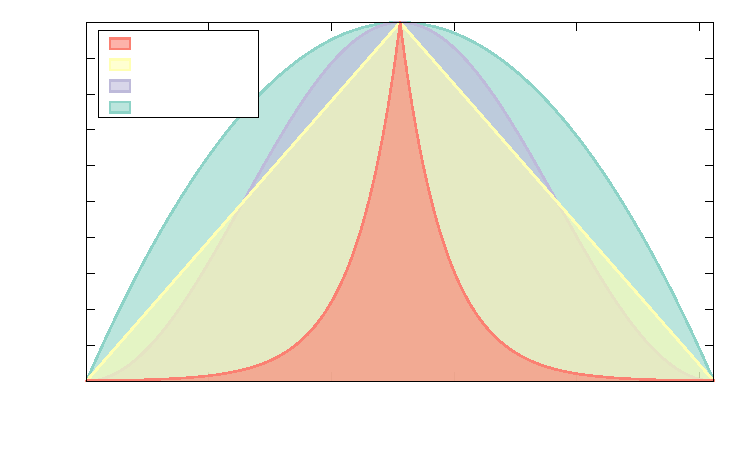
\includegraphics{graf4}}%
    \gplfronttext
  \end{picture}%
\endgroup
}
    \caption{Različne okenske funkcije.}
    \label{slika4}
\end{figure}
Okenske funkcije pomnožimo s~signalom v~časovnem prostoru in naredimo Fourierovo 
transformacijo. Na naslednjem grafu~\ref{slika5} so podatki obdelani z~okenskimi funkcijami.
Vidimo, da z~okensko funkcijo na prvih podatkih (na sliki levo) spekter le poslabšamo --
predvsem z~eksponentnim oknom vidimo, da amplitudo precej zmanjšamo in razširimo vrhove.
Na drugem spektru (na desni) za eksponentno okno opazimo podobno -- znižali smo vrhove in
jih razširili. Od ostalih oken se je najbolje izkazala \emph{Hannova} funkcija, ki je
vrhove zožala, vmesnemu območju pa se je precej zmanjšala amplituda.
\begin{figure}[H]
    \centering
    \resizebox{0.49\linewidth}{!}{% GNUPLOT: LaTeX picture with Postscript
\begingroup
  \makeatletter
  \providecommand\color[2][]{%
    \GenericError{(gnuplot) \space\space\space\@spaces}{%
      Package color not loaded in conjunction with
      terminal option `colourtext'%
    }{See the gnuplot documentation for explanation.%
    }{Either use 'blacktext' in gnuplot or load the package
      color.sty in LaTeX.}%
    \renewcommand\color[2][]{}%
  }%
  \providecommand\includegraphics[2][]{%
    \GenericError{(gnuplot) \space\space\space\@spaces}{%
      Package graphicx or graphics not loaded%
    }{See the gnuplot documentation for explanation.%
    }{The gnuplot epslatex terminal needs graphicx.sty or graphics.sty.}%
    \renewcommand\includegraphics[2][]{}%
  }%
  \providecommand\rotatebox[2]{#2}%
  \@ifundefined{ifGPcolor}{%
    \newif\ifGPcolor
    \GPcolortrue
  }{}%
  \@ifundefined{ifGPblacktext}{%
    \newif\ifGPblacktext
    \GPblacktexttrue
  }{}%
  % define a \g@addto@macro without @ in the name:
  \let\gplgaddtomacro\g@addto@macro
  % define empty templates for all commands taking text:
  \gdef\gplbacktext{}%
  \gdef\gplfronttext{}%
  \makeatother
  \ifGPblacktext
    % no textcolor at all
    \def\colorrgb#1{}%
    \def\colorgray#1{}%
  \else
    % gray or color?
    \ifGPcolor
      \def\colorrgb#1{\color[rgb]{#1}}%
      \def\colorgray#1{\color[gray]{#1}}%
      \expandafter\def\csname LTw\endcsname{\color{white}}%
      \expandafter\def\csname LTb\endcsname{\color{black}}%
      \expandafter\def\csname LTa\endcsname{\color{black}}%
      \expandafter\def\csname LT0\endcsname{\color[rgb]{1,0,0}}%
      \expandafter\def\csname LT1\endcsname{\color[rgb]{0,1,0}}%
      \expandafter\def\csname LT2\endcsname{\color[rgb]{0,0,1}}%
      \expandafter\def\csname LT3\endcsname{\color[rgb]{1,0,1}}%
      \expandafter\def\csname LT4\endcsname{\color[rgb]{0,1,1}}%
      \expandafter\def\csname LT5\endcsname{\color[rgb]{1,1,0}}%
      \expandafter\def\csname LT6\endcsname{\color[rgb]{0,0,0}}%
      \expandafter\def\csname LT7\endcsname{\color[rgb]{1,0.3,0}}%
      \expandafter\def\csname LT8\endcsname{\color[rgb]{0.5,0.5,0.5}}%
    \else
      % gray
      \def\colorrgb#1{\color{black}}%
      \def\colorgray#1{\color[gray]{#1}}%
      \expandafter\def\csname LTw\endcsname{\color{white}}%
      \expandafter\def\csname LTb\endcsname{\color{black}}%
      \expandafter\def\csname LTa\endcsname{\color{black}}%
      \expandafter\def\csname LT0\endcsname{\color{black}}%
      \expandafter\def\csname LT1\endcsname{\color{black}}%
      \expandafter\def\csname LT2\endcsname{\color{black}}%
      \expandafter\def\csname LT3\endcsname{\color{black}}%
      \expandafter\def\csname LT4\endcsname{\color{black}}%
      \expandafter\def\csname LT5\endcsname{\color{black}}%
      \expandafter\def\csname LT6\endcsname{\color{black}}%
      \expandafter\def\csname LT7\endcsname{\color{black}}%
      \expandafter\def\csname LT8\endcsname{\color{black}}%
    \fi
  \fi
    \setlength{\unitlength}{0.0500bp}%
    \ifx\gptboxheight\undefined%
      \newlength{\gptboxheight}%
      \newlength{\gptboxwidth}%
      \newsavebox{\gptboxtext}%
    \fi%
    \setlength{\fboxrule}{0.5pt}%
    \setlength{\fboxsep}{1pt}%
\begin{picture}(7200.00,5040.00)%
    \gplgaddtomacro\gplbacktext{%
      \csname LTb\endcsname%%
      \put(946,2533){\makebox(0,0)[r]{\strut{}$1$}}%
      \put(946,704){\makebox(0,0)[r]{\strut{}$10^{-4}$}}%
      \put(946,1161){\makebox(0,0)[r]{\strut{}$10^{-3}$}}%
      \put(946,1618){\makebox(0,0)[r]{\strut{}$10^{-2}$}}%
      \put(946,2076){\makebox(0,0)[r]{\strut{}$10^{-1}$}}%
      \put(946,2990){\makebox(0,0)[r]{\strut{}$10^{1}$}}%
      \put(946,3447){\makebox(0,0)[r]{\strut{}$10^{2}$}}%
      \put(946,3905){\makebox(0,0)[r]{\strut{}$10^{3}$}}%
      \put(946,4362){\makebox(0,0)[r]{\strut{}$10^{4}$}}%
      \put(946,4819){\makebox(0,0)[r]{\strut{}$10^{5}$}}%
      \put(1078,484){\makebox(0,0){\strut{}$0$}}%
      \put(2223,484){\makebox(0,0){\strut{}$0.1$}}%
      \put(3368,484){\makebox(0,0){\strut{}$0.2$}}%
      \put(4513,484){\makebox(0,0){\strut{}$0.3$}}%
      \put(5658,484){\makebox(0,0){\strut{}$0.4$}}%
      \put(6803,484){\makebox(0,0){\strut{}$0.5$}}%
    }%
    \gplgaddtomacro\gplfronttext{%
      \csname LTb\endcsname%%
      \put(209,2761){\rotatebox{-270}{\makebox(0,0){\strut{}$|f|^2$}}}%
      \put(3940,154){\makebox(0,0){\strut{}$\omega$}}%
      \csname LTb\endcsname%%
      \put(5615,3766){\makebox(0,0)[l]{\strut{}eksponent}}%
      \csname LTb\endcsname%%
      \put(5615,3986){\makebox(0,0)[l]{\strut{}Bartlett}}%
      \csname LTb\endcsname%%
      \put(5615,4206){\makebox(0,0)[l]{\strut{}Hann}}%
      \csname LTb\endcsname%%
      \put(5615,4426){\makebox(0,0)[l]{\strut{}Welch}}%
      \csname LTb\endcsname%%
      \put(5615,4646){\makebox(0,0)[l]{\strut{}brez okna}}%
    }%
    \gplbacktext
    \put(0,0){\includegraphics[width={360.00bp},height={252.00bp}]{graf5b}}%
    \gplfronttext
  \end{picture}%
\endgroup
}
    \resizebox{0.49\linewidth}{!}{% GNUPLOT: LaTeX picture with Postscript
\begingroup
  \makeatletter
  \providecommand\color[2][]{%
    \GenericError{(gnuplot) \space\space\space\@spaces}{%
      Package color not loaded in conjunction with
      terminal option `colourtext'%
    }{See the gnuplot documentation for explanation.%
    }{Either use 'blacktext' in gnuplot or load the package
      color.sty in LaTeX.}%
    \renewcommand\color[2][]{}%
  }%
  \providecommand\includegraphics[2][]{%
    \GenericError{(gnuplot) \space\space\space\@spaces}{%
      Package graphicx or graphics not loaded%
    }{See the gnuplot documentation for explanation.%
    }{The gnuplot epslatex terminal needs graphicx.sty or graphics.sty.}%
    \renewcommand\includegraphics[2][]{}%
  }%
  \providecommand\rotatebox[2]{#2}%
  \@ifundefined{ifGPcolor}{%
    \newif\ifGPcolor
    \GPcolortrue
  }{}%
  \@ifundefined{ifGPblacktext}{%
    \newif\ifGPblacktext
    \GPblacktexttrue
  }{}%
  % define a \g@addto@macro without @ in the name:
  \let\gplgaddtomacro\g@addto@macro
  % define empty templates for all commands taking text:
  \gdef\gplbacktext{}%
  \gdef\gplfronttext{}%
  \makeatother
  \ifGPblacktext
    % no textcolor at all
    \def\colorrgb#1{}%
    \def\colorgray#1{}%
  \else
    % gray or color?
    \ifGPcolor
      \def\colorrgb#1{\color[rgb]{#1}}%
      \def\colorgray#1{\color[gray]{#1}}%
      \expandafter\def\csname LTw\endcsname{\color{white}}%
      \expandafter\def\csname LTb\endcsname{\color{black}}%
      \expandafter\def\csname LTa\endcsname{\color{black}}%
      \expandafter\def\csname LT0\endcsname{\color[rgb]{1,0,0}}%
      \expandafter\def\csname LT1\endcsname{\color[rgb]{0,1,0}}%
      \expandafter\def\csname LT2\endcsname{\color[rgb]{0,0,1}}%
      \expandafter\def\csname LT3\endcsname{\color[rgb]{1,0,1}}%
      \expandafter\def\csname LT4\endcsname{\color[rgb]{0,1,1}}%
      \expandafter\def\csname LT5\endcsname{\color[rgb]{1,1,0}}%
      \expandafter\def\csname LT6\endcsname{\color[rgb]{0,0,0}}%
      \expandafter\def\csname LT7\endcsname{\color[rgb]{1,0.3,0}}%
      \expandafter\def\csname LT8\endcsname{\color[rgb]{0.5,0.5,0.5}}%
    \else
      % gray
      \def\colorrgb#1{\color{black}}%
      \def\colorgray#1{\color[gray]{#1}}%
      \expandafter\def\csname LTw\endcsname{\color{white}}%
      \expandafter\def\csname LTb\endcsname{\color{black}}%
      \expandafter\def\csname LTa\endcsname{\color{black}}%
      \expandafter\def\csname LT0\endcsname{\color{black}}%
      \expandafter\def\csname LT1\endcsname{\color{black}}%
      \expandafter\def\csname LT2\endcsname{\color{black}}%
      \expandafter\def\csname LT3\endcsname{\color{black}}%
      \expandafter\def\csname LT4\endcsname{\color{black}}%
      \expandafter\def\csname LT5\endcsname{\color{black}}%
      \expandafter\def\csname LT6\endcsname{\color{black}}%
      \expandafter\def\csname LT7\endcsname{\color{black}}%
      \expandafter\def\csname LT8\endcsname{\color{black}}%
    \fi
  \fi
    \setlength{\unitlength}{0.0500bp}%
    \ifx\gptboxheight\undefined%
      \newlength{\gptboxheight}%
      \newlength{\gptboxwidth}%
      \newsavebox{\gptboxtext}%
    \fi%
    \setlength{\fboxrule}{0.5pt}%
    \setlength{\fboxsep}{1pt}%
\begin{picture}(7200.00,5040.00)%
    \gplgaddtomacro\gplbacktext{%
      \csname LTb\endcsname%%
      \put(946,3055){\makebox(0,0)[r]{\strut{}$1$}}%
      \put(946,704){\makebox(0,0)[r]{\strut{}$10^{-8}$}}%
      \put(946,1292){\makebox(0,0)[r]{\strut{}$10^{-6}$}}%
      \put(946,1880){\makebox(0,0)[r]{\strut{}$10^{-4}$}}%
      \put(946,2468){\makebox(0,0)[r]{\strut{}$10^{-2}$}}%
      \put(946,3643){\makebox(0,0)[r]{\strut{}$10^{2}$}}%
      \put(946,4231){\makebox(0,0)[r]{\strut{}$10^{4}$}}%
      \put(946,4819){\makebox(0,0)[r]{\strut{}$10^{6}$}}%
      \put(1078,484){\makebox(0,0){\strut{}$0$}}%
      \put(2223,484){\makebox(0,0){\strut{}$0.1$}}%
      \put(3368,484){\makebox(0,0){\strut{}$0.2$}}%
      \put(4513,484){\makebox(0,0){\strut{}$0.3$}}%
      \put(5658,484){\makebox(0,0){\strut{}$0.4$}}%
      \put(6803,484){\makebox(0,0){\strut{}$0.5$}}%
    }%
    \gplgaddtomacro\gplfronttext{%
      \csname LTb\endcsname%%
      \put(209,2761){\rotatebox{-270}{\makebox(0,0){\strut{}$|f|^2$}}}%
      \put(3940,154){\makebox(0,0){\strut{}$\omega$}}%
      \csname LTb\endcsname%%
      \put(3642,877){\makebox(0,0)[l]{\strut{}eksponent}}%
      \csname LTb\endcsname%%
      \put(3642,1097){\makebox(0,0)[l]{\strut{}Bartlett}}%
      \csname LTb\endcsname%%
      \put(3642,1317){\makebox(0,0)[l]{\strut{}Hann}}%
      \csname LTb\endcsname%%
      \put(3642,1537){\makebox(0,0)[l]{\strut{}Welch}}%
      \csname LTb\endcsname%%
      \put(3642,1757){\makebox(0,0)[l]{\strut{}brez okna}}%
    }%
    \gplbacktext
    \put(0,0){\includegraphics[width={360.00bp},height={252.00bp}]{graf5a}}%
    \gplfronttext
  \end{picture}%
\endgroup
}
    \caption{Uporaba okenskih funkcij na obeh spektrih.}
    \label{slika5}
\end{figure}

\pagebreak

%----------------------------------------------------------------------------------------
%	PROBLEM 2
%----------------------------------------------------------------------------------------
\section{Wienerjev filter}
S~pomočjo Wienerjevega filtra naredimo dekonvolucijo signalov na datotekah 
\path{signal{0,1,2,3}.dat}. Število točk v~posameznem signalu je $512$. Na zadnjih treh 
datotekah je signalu primešan šum. Prenosna funkcija je
\begin{equation}
    r(t) = \frac{1}{2\tau} \mathrm{e}^{- |t|/\tau} \quad \tau=16.
\end{equation}
\subsection{Pristop}
Signal $u(t)$, ki prihaja v~merilno napravo s~prenosno funkcijo $r(t)$, se z~dodanim šumom
preoblikuje v:
\begin{equation}
    c(t) = (u*r)(t) + n(t) = s(t) + n(t),
\end{equation}
kjer je $s(t)$ izmerjen signal. Če šuma ni, lahko rekonstruiramo vhodni signal:
\begin{align}
    c(t) &= (u*r)(t) \quad 
    \xrightarrow{\mathcal{F}} \qquad 
    C(\omega) = U(\omega) \cdot R(\omega) \\
    U(\omega) &= \frac{C(\omega)}{R(\omega)} \qquad 
    \xrightarrow{\mathcal{F}^{-1}} \qquad 
    u(t) = \mathcal{F}^{-1}\left(\frac{C(\omega)}{R(\omega)}\right).
\end{align}
Ko dodamo šum moramo pred dekovolucijo transformiranko $C(\omega)$ pomnožiti z~Wienerjevim
filtrom:
\begin{equation}
    \Phi = \frac{|S(\omega)|^2}{|S(\omega)|^2 + |N(\omega)|^2},
\end{equation}
kjer sta $S(\omega)$ in $N(\omega)$ Fourierovi transformiranki $s(t)$ in $n(t)$.

\subsection{Reševanje in rezultati}
Na spodnjem grafu~\ref{slika6} so prikazani vsi štirje signali -- vidimo, da je prvi res
nezašumljen, ostali trije pa imajo precej šuma.
\begin{figure}[H]
    \centering
    \resizebox{0.49\linewidth}{!}{% GNUPLOT: LaTeX picture with Postscript
\begingroup
  \makeatletter
  \providecommand\color[2][]{%
    \GenericError{(gnuplot) \space\space\space\@spaces}{%
      Package color not loaded in conjunction with
      terminal option `colourtext'%
    }{See the gnuplot documentation for explanation.%
    }{Either use 'blacktext' in gnuplot or load the package
      color.sty in LaTeX.}%
    \renewcommand\color[2][]{}%
  }%
  \providecommand\includegraphics[2][]{%
    \GenericError{(gnuplot) \space\space\space\@spaces}{%
      Package graphicx or graphics not loaded%
    }{See the gnuplot documentation for explanation.%
    }{The gnuplot epslatex terminal needs graphicx.sty or graphics.sty.}%
    \renewcommand\includegraphics[2][]{}%
  }%
  \providecommand\rotatebox[2]{#2}%
  \@ifundefined{ifGPcolor}{%
    \newif\ifGPcolor
    \GPcolortrue
  }{}%
  \@ifundefined{ifGPblacktext}{%
    \newif\ifGPblacktext
    \GPblacktexttrue
  }{}%
  % define a \g@addto@macro without @ in the name:
  \let\gplgaddtomacro\g@addto@macro
  % define empty templates for all commands taking text:
  \gdef\gplbacktext{}%
  \gdef\gplfronttext{}%
  \makeatother
  \ifGPblacktext
    % no textcolor at all
    \def\colorrgb#1{}%
    \def\colorgray#1{}%
  \else
    % gray or color?
    \ifGPcolor
      \def\colorrgb#1{\color[rgb]{#1}}%
      \def\colorgray#1{\color[gray]{#1}}%
      \expandafter\def\csname LTw\endcsname{\color{white}}%
      \expandafter\def\csname LTb\endcsname{\color{black}}%
      \expandafter\def\csname LTa\endcsname{\color{black}}%
      \expandafter\def\csname LT0\endcsname{\color[rgb]{1,0,0}}%
      \expandafter\def\csname LT1\endcsname{\color[rgb]{0,1,0}}%
      \expandafter\def\csname LT2\endcsname{\color[rgb]{0,0,1}}%
      \expandafter\def\csname LT3\endcsname{\color[rgb]{1,0,1}}%
      \expandafter\def\csname LT4\endcsname{\color[rgb]{0,1,1}}%
      \expandafter\def\csname LT5\endcsname{\color[rgb]{1,1,0}}%
      \expandafter\def\csname LT6\endcsname{\color[rgb]{0,0,0}}%
      \expandafter\def\csname LT7\endcsname{\color[rgb]{1,0.3,0}}%
      \expandafter\def\csname LT8\endcsname{\color[rgb]{0.5,0.5,0.5}}%
    \else
      % gray
      \def\colorrgb#1{\color{black}}%
      \def\colorgray#1{\color[gray]{#1}}%
      \expandafter\def\csname LTw\endcsname{\color{white}}%
      \expandafter\def\csname LTb\endcsname{\color{black}}%
      \expandafter\def\csname LTa\endcsname{\color{black}}%
      \expandafter\def\csname LT0\endcsname{\color{black}}%
      \expandafter\def\csname LT1\endcsname{\color{black}}%
      \expandafter\def\csname LT2\endcsname{\color{black}}%
      \expandafter\def\csname LT3\endcsname{\color{black}}%
      \expandafter\def\csname LT4\endcsname{\color{black}}%
      \expandafter\def\csname LT5\endcsname{\color{black}}%
      \expandafter\def\csname LT6\endcsname{\color{black}}%
      \expandafter\def\csname LT7\endcsname{\color{black}}%
      \expandafter\def\csname LT8\endcsname{\color{black}}%
    \fi
  \fi
    \setlength{\unitlength}{0.0500bp}%
    \ifx\gptboxheight\undefined%
      \newlength{\gptboxheight}%
      \newlength{\gptboxwidth}%
      \newsavebox{\gptboxtext}%
    \fi%
    \setlength{\fboxrule}{0.5pt}%
    \setlength{\fboxsep}{1pt}%
\begin{picture}(7200.00,5040.00)%
    \gplgaddtomacro\gplbacktext{%
      \csname LTb\endcsname%%
      \put(462,440){\makebox(0,0)[r]{\strut{}$0$}}%
      \put(462,1316){\makebox(0,0)[r]{\strut{}$5$}}%
      \put(462,2192){\makebox(0,0)[r]{\strut{}$10$}}%
      \put(462,3067){\makebox(0,0)[r]{\strut{}$15$}}%
      \put(462,3943){\makebox(0,0)[r]{\strut{}$20$}}%
      \put(462,4819){\makebox(0,0)[r]{\strut{}$25$}}%
      \put(594,220){\makebox(0,0){\strut{}$0$}}%
      \put(1836,220){\makebox(0,0){\strut{}$2$}}%
      \put(3078,220){\makebox(0,0){\strut{}$4$}}%
      \put(4319,220){\makebox(0,0){\strut{}$6$}}%
      \put(5561,220){\makebox(0,0){\strut{}$8$}}%
      \put(6803,220){\makebox(0,0){\strut{}$10$}}%
    }%
    \gplgaddtomacro\gplfronttext{%
      \csname LTb\endcsname%%
      \put(5086,3216){\makebox(0,0)[l]{\strut{}$ \Delta t = 0.001$}}%
      \csname LTb\endcsname%%
      \put(5086,3436){\makebox(0,0)[l]{\strut{}$ \Delta t = 0.01$}}%
      \csname LTb\endcsname%%
      \put(5086,3656){\makebox(0,0)[l]{\strut{}$ \Delta t = 0.1$}}%
      \csname LTb\endcsname%%
      \put(5086,3876){\makebox(0,0)[l]{\strut{}$ \Delta t = 0.25$}}%
      \csname LTb\endcsname%%
      \put(5086,4096){\makebox(0,0)[l]{\strut{}$ \Delta t = 0.5$}}%
      \csname LTb\endcsname%%
      \put(5086,4316){\makebox(0,0)[l]{\strut{}$ \Delta t = 1$}}%
      \csname LTb\endcsname%%
      \put(5086,4536){\makebox(0,0)[l]{\strut{}$N_0 \mathrm{e}^{-\beta t}$}}%
    }%
    \gplbacktext
    \put(0,0){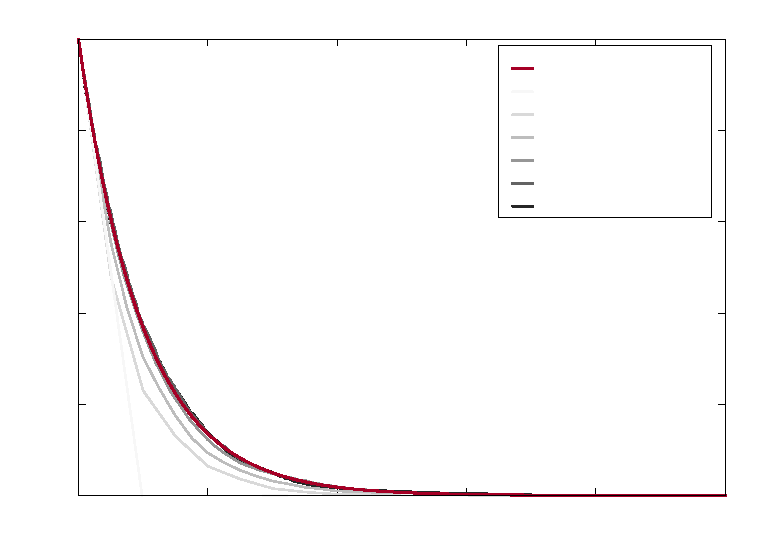
\includegraphics[width={360.00bp},height={252.00bp}]{graf6}}%
    \gplfronttext
  \end{picture}%
\endgroup
}
    \resizebox{0.49\linewidth}{!}{% GNUPLOT: LaTeX picture with Postscript
\begingroup
  \makeatletter
  \providecommand\color[2][]{%
    \GenericError{(gnuplot) \space\space\space\@spaces}{%
      Package color not loaded in conjunction with
      terminal option `colourtext'%
    }{See the gnuplot documentation for explanation.%
    }{Either use 'blacktext' in gnuplot or load the package
      color.sty in LaTeX.}%
    \renewcommand\color[2][]{}%
  }%
  \providecommand\includegraphics[2][]{%
    \GenericError{(gnuplot) \space\space\space\@spaces}{%
      Package graphicx or graphics not loaded%
    }{See the gnuplot documentation for explanation.%
    }{The gnuplot epslatex terminal needs graphicx.sty or graphics.sty.}%
    \renewcommand\includegraphics[2][]{}%
  }%
  \providecommand\rotatebox[2]{#2}%
  \@ifundefined{ifGPcolor}{%
    \newif\ifGPcolor
    \GPcolortrue
  }{}%
  \@ifundefined{ifGPblacktext}{%
    \newif\ifGPblacktext
    \GPblacktexttrue
  }{}%
  % define a \g@addto@macro without @ in the name:
  \let\gplgaddtomacro\g@addto@macro
  % define empty templates for all commands taking text:
  \gdef\gplbacktext{}%
  \gdef\gplfronttext{}%
  \makeatother
  \ifGPblacktext
    % no textcolor at all
    \def\colorrgb#1{}%
    \def\colorgray#1{}%
  \else
    % gray or color?
    \ifGPcolor
      \def\colorrgb#1{\color[rgb]{#1}}%
      \def\colorgray#1{\color[gray]{#1}}%
      \expandafter\def\csname LTw\endcsname{\color{white}}%
      \expandafter\def\csname LTb\endcsname{\color{black}}%
      \expandafter\def\csname LTa\endcsname{\color{black}}%
      \expandafter\def\csname LT0\endcsname{\color[rgb]{1,0,0}}%
      \expandafter\def\csname LT1\endcsname{\color[rgb]{0,1,0}}%
      \expandafter\def\csname LT2\endcsname{\color[rgb]{0,0,1}}%
      \expandafter\def\csname LT3\endcsname{\color[rgb]{1,0,1}}%
      \expandafter\def\csname LT4\endcsname{\color[rgb]{0,1,1}}%
      \expandafter\def\csname LT5\endcsname{\color[rgb]{1,1,0}}%
      \expandafter\def\csname LT6\endcsname{\color[rgb]{0,0,0}}%
      \expandafter\def\csname LT7\endcsname{\color[rgb]{1,0.3,0}}%
      \expandafter\def\csname LT8\endcsname{\color[rgb]{0.5,0.5,0.5}}%
    \else
      % gray
      \def\colorrgb#1{\color{black}}%
      \def\colorgray#1{\color[gray]{#1}}%
      \expandafter\def\csname LTw\endcsname{\color{white}}%
      \expandafter\def\csname LTb\endcsname{\color{black}}%
      \expandafter\def\csname LTa\endcsname{\color{black}}%
      \expandafter\def\csname LT0\endcsname{\color{black}}%
      \expandafter\def\csname LT1\endcsname{\color{black}}%
      \expandafter\def\csname LT2\endcsname{\color{black}}%
      \expandafter\def\csname LT3\endcsname{\color{black}}%
      \expandafter\def\csname LT4\endcsname{\color{black}}%
      \expandafter\def\csname LT5\endcsname{\color{black}}%
      \expandafter\def\csname LT6\endcsname{\color{black}}%
      \expandafter\def\csname LT7\endcsname{\color{black}}%
      \expandafter\def\csname LT8\endcsname{\color{black}}%
    \fi
  \fi
    \setlength{\unitlength}{0.0500bp}%
    \ifx\gptboxheight\undefined%
      \newlength{\gptboxheight}%
      \newlength{\gptboxwidth}%
      \newsavebox{\gptboxtext}%
    \fi%
    \setlength{\fboxrule}{0.5pt}%
    \setlength{\fboxsep}{1pt}%
\begin{picture}(7200.00,5040.00)%
    \gplgaddtomacro\gplbacktext{%
    }%
    \gplgaddtomacro\gplfronttext{%
      \csname LTb\endcsname%%
      \put(3566,4709){\makebox(0,0){\strut{}$T=0.5$}}%
    }%
    \gplbacktext
    \put(0,0){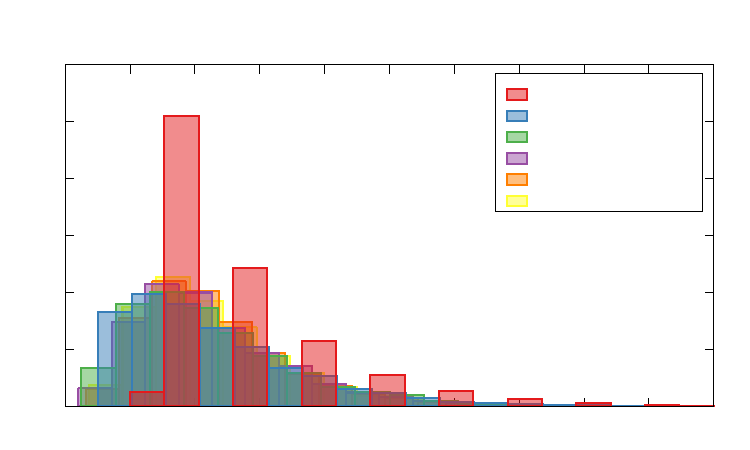
\includegraphics{graf10}}%
    \gplfronttext
  \end{picture}%
\endgroup
}
    \caption{Na levi je prikazan prvi signal -- $c_0$, na desni pa ostali trije signali.}
    \label{slika6}
\end{figure}
Zgoraj omenjeni postopek najprej uporabimo na nezašumljenem signalu \path{signal0} in 
poskusimo dobiti iz njega vhodni signal $u_0$. Na grafu~\ref{slika7} levo vidimo njegov
frekvenčni spekter, na desni pa rekonstruiran vstopni signal. Ta je sestavljen iz štirih
škatlastih signalov -- prvi je najvišji in najožji, ostali pa se nato nižajo in širijo.
\begin{figure}[H]
    \centering
    \resizebox{0.49\linewidth}{!}{% GNUPLOT: LaTeX picture with Postscript
\begingroup
  \makeatletter
  \providecommand\color[2][]{%
    \GenericError{(gnuplot) \space\space\space\@spaces}{%
      Package color not loaded in conjunction with
      terminal option `colourtext'%
    }{See the gnuplot documentation for explanation.%
    }{Either use 'blacktext' in gnuplot or load the package
      color.sty in LaTeX.}%
    \renewcommand\color[2][]{}%
  }%
  \providecommand\includegraphics[2][]{%
    \GenericError{(gnuplot) \space\space\space\@spaces}{%
      Package graphicx or graphics not loaded%
    }{See the gnuplot documentation for explanation.%
    }{The gnuplot epslatex terminal needs graphicx.sty or graphics.sty.}%
    \renewcommand\includegraphics[2][]{}%
  }%
  \providecommand\rotatebox[2]{#2}%
  \@ifundefined{ifGPcolor}{%
    \newif\ifGPcolor
    \GPcolortrue
  }{}%
  \@ifundefined{ifGPblacktext}{%
    \newif\ifGPblacktext
    \GPblacktexttrue
  }{}%
  % define a \g@addto@macro without @ in the name:
  \let\gplgaddtomacro\g@addto@macro
  % define empty templates for all commands taking text:
  \gdef\gplbacktext{}%
  \gdef\gplfronttext{}%
  \makeatother
  \ifGPblacktext
    % no textcolor at all
    \def\colorrgb#1{}%
    \def\colorgray#1{}%
  \else
    % gray or color?
    \ifGPcolor
      \def\colorrgb#1{\color[rgb]{#1}}%
      \def\colorgray#1{\color[gray]{#1}}%
      \expandafter\def\csname LTw\endcsname{\color{white}}%
      \expandafter\def\csname LTb\endcsname{\color{black}}%
      \expandafter\def\csname LTa\endcsname{\color{black}}%
      \expandafter\def\csname LT0\endcsname{\color[rgb]{1,0,0}}%
      \expandafter\def\csname LT1\endcsname{\color[rgb]{0,1,0}}%
      \expandafter\def\csname LT2\endcsname{\color[rgb]{0,0,1}}%
      \expandafter\def\csname LT3\endcsname{\color[rgb]{1,0,1}}%
      \expandafter\def\csname LT4\endcsname{\color[rgb]{0,1,1}}%
      \expandafter\def\csname LT5\endcsname{\color[rgb]{1,1,0}}%
      \expandafter\def\csname LT6\endcsname{\color[rgb]{0,0,0}}%
      \expandafter\def\csname LT7\endcsname{\color[rgb]{1,0.3,0}}%
      \expandafter\def\csname LT8\endcsname{\color[rgb]{0.5,0.5,0.5}}%
    \else
      % gray
      \def\colorrgb#1{\color{black}}%
      \def\colorgray#1{\color[gray]{#1}}%
      \expandafter\def\csname LTw\endcsname{\color{white}}%
      \expandafter\def\csname LTb\endcsname{\color{black}}%
      \expandafter\def\csname LTa\endcsname{\color{black}}%
      \expandafter\def\csname LT0\endcsname{\color{black}}%
      \expandafter\def\csname LT1\endcsname{\color{black}}%
      \expandafter\def\csname LT2\endcsname{\color{black}}%
      \expandafter\def\csname LT3\endcsname{\color{black}}%
      \expandafter\def\csname LT4\endcsname{\color{black}}%
      \expandafter\def\csname LT5\endcsname{\color{black}}%
      \expandafter\def\csname LT6\endcsname{\color{black}}%
      \expandafter\def\csname LT7\endcsname{\color{black}}%
      \expandafter\def\csname LT8\endcsname{\color{black}}%
    \fi
  \fi
    \setlength{\unitlength}{0.0500bp}%
    \ifx\gptboxheight\undefined%
      \newlength{\gptboxheight}%
      \newlength{\gptboxwidth}%
      \newsavebox{\gptboxtext}%
    \fi%
    \setlength{\fboxrule}{0.5pt}%
    \setlength{\fboxsep}{1pt}%
\begin{picture}(7200.00,4320.00)%
    \gplgaddtomacro\gplbacktext{%
      \csname LTb\endcsname%%
      \put(504,408){\makebox(0,0)[r]{\strut{}$0$}}%
      \csname LTb\endcsname%%
      \put(504,954){\makebox(0,0)[r]{\strut{}$0.1$}}%
      \csname LTb\endcsname%%
      \put(504,1501){\makebox(0,0)[r]{\strut{}$0.2$}}%
      \csname LTb\endcsname%%
      \put(504,2048){\makebox(0,0)[r]{\strut{}$0.3$}}%
      \csname LTb\endcsname%%
      \put(504,2594){\makebox(0,0)[r]{\strut{}$0.4$}}%
      \csname LTb\endcsname%%
      \put(504,3140){\makebox(0,0)[r]{\strut{}$0.5$}}%
      \csname LTb\endcsname%%
      \put(504,3687){\makebox(0,0)[r]{\strut{}$0.6$}}%
      \csname LTb\endcsname%%
      \put(616,204){\makebox(0,0){\strut{}$0$}}%
      \csname LTb\endcsname%%
      \put(1239,204){\makebox(0,0){\strut{}$1$}}%
      \csname LTb\endcsname%%
      \put(1861,204){\makebox(0,0){\strut{}$2$}}%
      \csname LTb\endcsname%%
      \put(2484,204){\makebox(0,0){\strut{}$3$}}%
      \csname LTb\endcsname%%
      \put(3107,204){\makebox(0,0){\strut{}$4$}}%
      \csname LTb\endcsname%%
      \put(3730,204){\makebox(0,0){\strut{}$5$}}%
      \csname LTb\endcsname%%
      \put(4352,204){\makebox(0,0){\strut{}$6$}}%
      \csname LTb\endcsname%%
      \put(4975,204){\makebox(0,0){\strut{}$7$}}%
      \csname LTb\endcsname%%
      \put(5598,204){\makebox(0,0){\strut{}$8$}}%
      \csname LTb\endcsname%%
      \put(6220,204){\makebox(0,0){\strut{}$9$}}%
      \csname LTb\endcsname%%
      \put(6843,204){\makebox(0,0){\strut{}$10$}}%
    }%
    \gplgaddtomacro\gplfronttext{%
      \csname LTb\endcsname%%
      \put(5163,2382){\makebox(0,0)[l]{\strut{}$ \Delta t = 0.001$}}%
      \csname LTb\endcsname%%
      \put(5163,2586){\makebox(0,0)[l]{\strut{}$ \Delta t = 0.01$}}%
      \csname LTb\endcsname%%
      \put(5163,2790){\makebox(0,0)[l]{\strut{}$ \Delta t = 0.1$}}%
      \csname LTb\endcsname%%
      \put(5163,2994){\makebox(0,0)[l]{\strut{}$ \Delta t = 0.25$}}%
      \csname LTb\endcsname%%
      \put(5163,3198){\makebox(0,0)[l]{\strut{}$ \Delta t = 0.5$}}%
      \csname LTb\endcsname%%
      \put(5163,3402){\makebox(0,0)[l]{\strut{}$ \Delta t = 1$}}%
      \csname LTb\endcsname%%
      \put(3729,3993){\makebox(0,0){\strut{}$N_0 = 250$}}%
    }%
    \gplbacktext
    \put(0,0){\includegraphics[width={360.00bp},height={216.00bp}]{graf11}}%
    \gplfronttext
  \end{picture}%
\endgroup
}
    \resizebox{0.49\linewidth}{!}{% GNUPLOT: LaTeX picture with Postscript
\begingroup
  \makeatletter
  \providecommand\color[2][]{%
    \GenericError{(gnuplot) \space\space\space\@spaces}{%
      Package color not loaded in conjunction with
      terminal option `colourtext'%
    }{See the gnuplot documentation for explanation.%
    }{Either use 'blacktext' in gnuplot or load the package
      color.sty in LaTeX.}%
    \renewcommand\color[2][]{}%
  }%
  \providecommand\includegraphics[2][]{%
    \GenericError{(gnuplot) \space\space\space\@spaces}{%
      Package graphicx or graphics not loaded%
    }{See the gnuplot documentation for explanation.%
    }{The gnuplot epslatex terminal needs graphicx.sty or graphics.sty.}%
    \renewcommand\includegraphics[2][]{}%
  }%
  \providecommand\rotatebox[2]{#2}%
  \@ifundefined{ifGPcolor}{%
    \newif\ifGPcolor
    \GPcolortrue
  }{}%
  \@ifundefined{ifGPblacktext}{%
    \newif\ifGPblacktext
    \GPblacktexttrue
  }{}%
  % define a \g@addto@macro without @ in the name:
  \let\gplgaddtomacro\g@addto@macro
  % define empty templates for all commands taking text:
  \gdef\gplbacktext{}%
  \gdef\gplfronttext{}%
  \makeatother
  \ifGPblacktext
    % no textcolor at all
    \def\colorrgb#1{}%
    \def\colorgray#1{}%
  \else
    % gray or color?
    \ifGPcolor
      \def\colorrgb#1{\color[rgb]{#1}}%
      \def\colorgray#1{\color[gray]{#1}}%
      \expandafter\def\csname LTw\endcsname{\color{white}}%
      \expandafter\def\csname LTb\endcsname{\color{black}}%
      \expandafter\def\csname LTa\endcsname{\color{black}}%
      \expandafter\def\csname LT0\endcsname{\color[rgb]{1,0,0}}%
      \expandafter\def\csname LT1\endcsname{\color[rgb]{0,1,0}}%
      \expandafter\def\csname LT2\endcsname{\color[rgb]{0,0,1}}%
      \expandafter\def\csname LT3\endcsname{\color[rgb]{1,0,1}}%
      \expandafter\def\csname LT4\endcsname{\color[rgb]{0,1,1}}%
      \expandafter\def\csname LT5\endcsname{\color[rgb]{1,1,0}}%
      \expandafter\def\csname LT6\endcsname{\color[rgb]{0,0,0}}%
      \expandafter\def\csname LT7\endcsname{\color[rgb]{1,0.3,0}}%
      \expandafter\def\csname LT8\endcsname{\color[rgb]{0.5,0.5,0.5}}%
    \else
      % gray
      \def\colorrgb#1{\color{black}}%
      \def\colorgray#1{\color[gray]{#1}}%
      \expandafter\def\csname LTw\endcsname{\color{white}}%
      \expandafter\def\csname LTb\endcsname{\color{black}}%
      \expandafter\def\csname LTa\endcsname{\color{black}}%
      \expandafter\def\csname LT0\endcsname{\color{black}}%
      \expandafter\def\csname LT1\endcsname{\color{black}}%
      \expandafter\def\csname LT2\endcsname{\color{black}}%
      \expandafter\def\csname LT3\endcsname{\color{black}}%
      \expandafter\def\csname LT4\endcsname{\color{black}}%
      \expandafter\def\csname LT5\endcsname{\color{black}}%
      \expandafter\def\csname LT6\endcsname{\color{black}}%
      \expandafter\def\csname LT7\endcsname{\color{black}}%
      \expandafter\def\csname LT8\endcsname{\color{black}}%
    \fi
  \fi
    \setlength{\unitlength}{0.0500bp}%
    \ifx\gptboxheight\undefined%
      \newlength{\gptboxheight}%
      \newlength{\gptboxwidth}%
      \newsavebox{\gptboxtext}%
    \fi%
    \setlength{\fboxrule}{0.5pt}%
    \setlength{\fboxsep}{1pt}%
\begin{picture}(7200.00,4320.00)%
    \gplgaddtomacro\gplbacktext{%
      \csname LTb\endcsname%%
      \put(504,408){\makebox(0,0)[r]{\strut{}$0$}}%
      \csname LTb\endcsname%%
      \put(504,954){\makebox(0,0)[r]{\strut{}$0.1$}}%
      \csname LTb\endcsname%%
      \put(504,1501){\makebox(0,0)[r]{\strut{}$0.2$}}%
      \csname LTb\endcsname%%
      \put(504,2048){\makebox(0,0)[r]{\strut{}$0.3$}}%
      \csname LTb\endcsname%%
      \put(504,2594){\makebox(0,0)[r]{\strut{}$0.4$}}%
      \csname LTb\endcsname%%
      \put(504,3140){\makebox(0,0)[r]{\strut{}$0.5$}}%
      \csname LTb\endcsname%%
      \put(504,3687){\makebox(0,0)[r]{\strut{}$0.6$}}%
      \csname LTb\endcsname%%
      \put(616,204){\makebox(0,0){\strut{}$0$}}%
      \csname LTb\endcsname%%
      \put(1308,204){\makebox(0,0){\strut{}$1$}}%
      \csname LTb\endcsname%%
      \put(2000,204){\makebox(0,0){\strut{}$2$}}%
      \csname LTb\endcsname%%
      \put(2692,204){\makebox(0,0){\strut{}$3$}}%
      \csname LTb\endcsname%%
      \put(3384,204){\makebox(0,0){\strut{}$4$}}%
      \csname LTb\endcsname%%
      \put(4075,204){\makebox(0,0){\strut{}$5$}}%
      \csname LTb\endcsname%%
      \put(4767,204){\makebox(0,0){\strut{}$6$}}%
      \csname LTb\endcsname%%
      \put(5459,204){\makebox(0,0){\strut{}$7$}}%
      \csname LTb\endcsname%%
      \put(6151,204){\makebox(0,0){\strut{}$8$}}%
      \csname LTb\endcsname%%
      \put(6843,204){\makebox(0,0){\strut{}$9$}}%
    }%
    \gplgaddtomacro\gplfronttext{%
      \csname LTb\endcsname%%
      \put(5163,2382){\makebox(0,0)[l]{\strut{}$ \Delta t = 0.001$}}%
      \csname LTb\endcsname%%
      \put(5163,2586){\makebox(0,0)[l]{\strut{}$ \Delta t = 0.01$}}%
      \csname LTb\endcsname%%
      \put(5163,2790){\makebox(0,0)[l]{\strut{}$ \Delta t = 0.1$}}%
      \csname LTb\endcsname%%
      \put(5163,2994){\makebox(0,0)[l]{\strut{}$ \Delta t = 0.25$}}%
      \csname LTb\endcsname%%
      \put(5163,3198){\makebox(0,0)[l]{\strut{}$ \Delta t = 0.5$}}%
      \csname LTb\endcsname%%
      \put(5163,3402){\makebox(0,0)[l]{\strut{}$ \Delta t = 1$}}%
      \csname LTb\endcsname%%
      \put(3729,3993){\makebox(0,0){\strut{}$N_0 = 25$}}%
    }%
    \gplbacktext
    \put(0,0){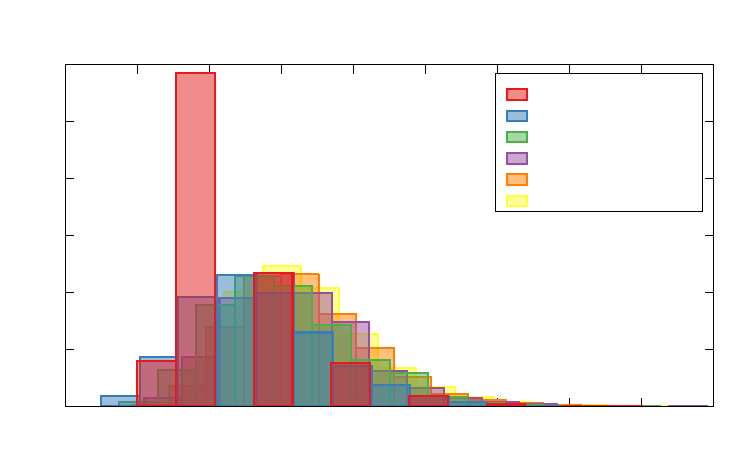
\includegraphics[width={360.00bp},height={216.00bp}]{graf8}}%
    \gplfronttext
  \end{picture}%
\endgroup
}
    \caption{Frekvenčni spekter signala $c_0$ in dekonvuliran vstopni signal $u_0(t)$.}
    \label{slika7}
\end{figure}
Z~Wienerjevim filtrom rekonstruiramo še ostale signale in dobimo graf~\ref{slika8}. Moči
vsakega spektra so vedno višje, dobljen vhodni signal pa kljub uporabi filtra ni podoben
nezašumljenem signalu.
\begin{figure}[H]
    \centering
    \resizebox{0.49\linewidth}{!}{% GNUPLOT: LaTeX picture with Postscript
\begingroup
  \makeatletter
  \providecommand\color[2][]{%
    \GenericError{(gnuplot) \space\space\space\@spaces}{%
      Package color not loaded in conjunction with
      terminal option `colourtext'%
    }{See the gnuplot documentation for explanation.%
    }{Either use 'blacktext' in gnuplot or load the package
      color.sty in LaTeX.}%
    \renewcommand\color[2][]{}%
  }%
  \providecommand\includegraphics[2][]{%
    \GenericError{(gnuplot) \space\space\space\@spaces}{%
      Package graphicx or graphics not loaded%
    }{See the gnuplot documentation for explanation.%
    }{The gnuplot epslatex terminal needs graphicx.sty or graphics.sty.}%
    \renewcommand\includegraphics[2][]{}%
  }%
  \providecommand\rotatebox[2]{#2}%
  \@ifundefined{ifGPcolor}{%
    \newif\ifGPcolor
    \GPcolortrue
  }{}%
  \@ifundefined{ifGPblacktext}{%
    \newif\ifGPblacktext
    \GPblacktexttrue
  }{}%
  % define a \g@addto@macro without @ in the name:
  \let\gplgaddtomacro\g@addto@macro
  % define empty templates for all commands taking text:
  \gdef\gplbacktext{}%
  \gdef\gplfronttext{}%
  \makeatother
  \ifGPblacktext
    % no textcolor at all
    \def\colorrgb#1{}%
    \def\colorgray#1{}%
  \else
    % gray or color?
    \ifGPcolor
      \def\colorrgb#1{\color[rgb]{#1}}%
      \def\colorgray#1{\color[gray]{#1}}%
      \expandafter\def\csname LTw\endcsname{\color{white}}%
      \expandafter\def\csname LTb\endcsname{\color{black}}%
      \expandafter\def\csname LTa\endcsname{\color{black}}%
      \expandafter\def\csname LT0\endcsname{\color[rgb]{1,0,0}}%
      \expandafter\def\csname LT1\endcsname{\color[rgb]{0,1,0}}%
      \expandafter\def\csname LT2\endcsname{\color[rgb]{0,0,1}}%
      \expandafter\def\csname LT3\endcsname{\color[rgb]{1,0,1}}%
      \expandafter\def\csname LT4\endcsname{\color[rgb]{0,1,1}}%
      \expandafter\def\csname LT5\endcsname{\color[rgb]{1,1,0}}%
      \expandafter\def\csname LT6\endcsname{\color[rgb]{0,0,0}}%
      \expandafter\def\csname LT7\endcsname{\color[rgb]{1,0.3,0}}%
      \expandafter\def\csname LT8\endcsname{\color[rgb]{0.5,0.5,0.5}}%
    \else
      % gray
      \def\colorrgb#1{\color{black}}%
      \def\colorgray#1{\color[gray]{#1}}%
      \expandafter\def\csname LTw\endcsname{\color{white}}%
      \expandafter\def\csname LTb\endcsname{\color{black}}%
      \expandafter\def\csname LTa\endcsname{\color{black}}%
      \expandafter\def\csname LT0\endcsname{\color{black}}%
      \expandafter\def\csname LT1\endcsname{\color{black}}%
      \expandafter\def\csname LT2\endcsname{\color{black}}%
      \expandafter\def\csname LT3\endcsname{\color{black}}%
      \expandafter\def\csname LT4\endcsname{\color{black}}%
      \expandafter\def\csname LT5\endcsname{\color{black}}%
      \expandafter\def\csname LT6\endcsname{\color{black}}%
      \expandafter\def\csname LT7\endcsname{\color{black}}%
      \expandafter\def\csname LT8\endcsname{\color{black}}%
    \fi
  \fi
    \setlength{\unitlength}{0.0500bp}%
    \ifx\gptboxheight\undefined%
      \newlength{\gptboxheight}%
      \newlength{\gptboxwidth}%
      \newsavebox{\gptboxtext}%
    \fi%
    \setlength{\fboxrule}{0.5pt}%
    \setlength{\fboxsep}{1pt}%
\begin{picture}(7200.00,5040.00)%
    \gplgaddtomacro\gplbacktext{%
      \csname LTb\endcsname%%
      \put(594,440){\makebox(0,0)[r]{\strut{}$0.1$}}%
      \put(594,1900){\makebox(0,0)[r]{\strut{}$1$}}%
      \put(594,3359){\makebox(0,0)[r]{\strut{}$10$}}%
      \put(594,4819){\makebox(0,0)[r]{\strut{}$100$}}%
      \put(726,220){\makebox(0,0){\strut{}$0$}}%
      \put(1941,220){\makebox(0,0){\strut{}$2$}}%
      \put(3157,220){\makebox(0,0){\strut{}$4$}}%
      \put(4372,220){\makebox(0,0){\strut{}$6$}}%
      \put(5588,220){\makebox(0,0){\strut{}$8$}}%
      \put(6803,220){\makebox(0,0){\strut{}$10$}}%
    }%
    \gplgaddtomacro\gplfronttext{%
      \csname LTb\endcsname%%
      \put(5086,3216){\makebox(0,0)[l]{\strut{}$ \Delta t = 0.001$}}%
      \csname LTb\endcsname%%
      \put(5086,3436){\makebox(0,0)[l]{\strut{}$ \Delta t = 0.01$}}%
      \csname LTb\endcsname%%
      \put(5086,3656){\makebox(0,0)[l]{\strut{}$ \Delta t = 0.1$}}%
      \csname LTb\endcsname%%
      \put(5086,3876){\makebox(0,0)[l]{\strut{}$ \Delta t = 0.25$}}%
      \csname LTb\endcsname%%
      \put(5086,4096){\makebox(0,0)[l]{\strut{}$ \Delta t = 0.5$}}%
      \csname LTb\endcsname%%
      \put(5086,4316){\makebox(0,0)[l]{\strut{}$ \Delta t = 1$}}%
      \csname LTb\endcsname%%
      \put(5086,4536){\makebox(0,0)[l]{\strut{}$N_0 \mathrm{e}^{-\beta t}$}}%
    }%
    \gplbacktext
    \put(0,0){\includegraphics[width={360.00bp},height={252.00bp}]{graf7}}%
    \gplfronttext
  \end{picture}%
\endgroup
}
    \resizebox{0.49\linewidth}{!}{% GNUPLOT: LaTeX picture with Postscript
\begingroup
  \makeatletter
  \providecommand\color[2][]{%
    \GenericError{(gnuplot) \space\space\space\@spaces}{%
      Package color not loaded in conjunction with
      terminal option `colourtext'%
    }{See the gnuplot documentation for explanation.%
    }{Either use 'blacktext' in gnuplot or load the package
      color.sty in LaTeX.}%
    \renewcommand\color[2][]{}%
  }%
  \providecommand\includegraphics[2][]{%
    \GenericError{(gnuplot) \space\space\space\@spaces}{%
      Package graphicx or graphics not loaded%
    }{See the gnuplot documentation for explanation.%
    }{The gnuplot epslatex terminal needs graphicx.sty or graphics.sty.}%
    \renewcommand\includegraphics[2][]{}%
  }%
  \providecommand\rotatebox[2]{#2}%
  \@ifundefined{ifGPcolor}{%
    \newif\ifGPcolor
    \GPcolortrue
  }{}%
  \@ifundefined{ifGPblacktext}{%
    \newif\ifGPblacktext
    \GPblacktexttrue
  }{}%
  % define a \g@addto@macro without @ in the name:
  \let\gplgaddtomacro\g@addto@macro
  % define empty templates for all commands taking text:
  \gdef\gplbacktext{}%
  \gdef\gplfronttext{}%
  \makeatother
  \ifGPblacktext
    % no textcolor at all
    \def\colorrgb#1{}%
    \def\colorgray#1{}%
  \else
    % gray or color?
    \ifGPcolor
      \def\colorrgb#1{\color[rgb]{#1}}%
      \def\colorgray#1{\color[gray]{#1}}%
      \expandafter\def\csname LTw\endcsname{\color{white}}%
      \expandafter\def\csname LTb\endcsname{\color{black}}%
      \expandafter\def\csname LTa\endcsname{\color{black}}%
      \expandafter\def\csname LT0\endcsname{\color[rgb]{1,0,0}}%
      \expandafter\def\csname LT1\endcsname{\color[rgb]{0,1,0}}%
      \expandafter\def\csname LT2\endcsname{\color[rgb]{0,0,1}}%
      \expandafter\def\csname LT3\endcsname{\color[rgb]{1,0,1}}%
      \expandafter\def\csname LT4\endcsname{\color[rgb]{0,1,1}}%
      \expandafter\def\csname LT5\endcsname{\color[rgb]{1,1,0}}%
      \expandafter\def\csname LT6\endcsname{\color[rgb]{0,0,0}}%
      \expandafter\def\csname LT7\endcsname{\color[rgb]{1,0.3,0}}%
      \expandafter\def\csname LT8\endcsname{\color[rgb]{0.5,0.5,0.5}}%
    \else
      % gray
      \def\colorrgb#1{\color{black}}%
      \def\colorgray#1{\color[gray]{#1}}%
      \expandafter\def\csname LTw\endcsname{\color{white}}%
      \expandafter\def\csname LTb\endcsname{\color{black}}%
      \expandafter\def\csname LTa\endcsname{\color{black}}%
      \expandafter\def\csname LT0\endcsname{\color{black}}%
      \expandafter\def\csname LT1\endcsname{\color{black}}%
      \expandafter\def\csname LT2\endcsname{\color{black}}%
      \expandafter\def\csname LT3\endcsname{\color{black}}%
      \expandafter\def\csname LT4\endcsname{\color{black}}%
      \expandafter\def\csname LT5\endcsname{\color{black}}%
      \expandafter\def\csname LT6\endcsname{\color{black}}%
      \expandafter\def\csname LT7\endcsname{\color{black}}%
      \expandafter\def\csname LT8\endcsname{\color{black}}%
    \fi
  \fi
    \setlength{\unitlength}{0.0500bp}%
    \ifx\gptboxheight\undefined%
      \newlength{\gptboxheight}%
      \newlength{\gptboxwidth}%
      \newsavebox{\gptboxtext}%
    \fi%
    \setlength{\fboxrule}{0.5pt}%
    \setlength{\fboxsep}{1pt}%
\begin{picture}(7200.00,5040.00)%
    \gplgaddtomacro\gplbacktext{%
      \csname LTb\endcsname%%
      \put(682,704){\makebox(0,0)[r]{\strut{}$-3$}}%
      \put(682,1292){\makebox(0,0)[r]{\strut{}$-2$}}%
      \put(682,1880){\makebox(0,0)[r]{\strut{}$-1$}}%
      \put(682,2468){\makebox(0,0)[r]{\strut{}$0$}}%
      \put(682,3055){\makebox(0,0)[r]{\strut{}$1$}}%
      \put(682,3643){\makebox(0,0)[r]{\strut{}$2$}}%
      \put(682,4231){\makebox(0,0)[r]{\strut{}$3$}}%
      \put(682,4819){\makebox(0,0)[r]{\strut{}$4$}}%
      \put(814,484){\makebox(0,0){\strut{}$0$}}%
      \put(1984,484){\makebox(0,0){\strut{}$100$}}%
      \put(3153,484){\makebox(0,0){\strut{}$200$}}%
      \put(4323,484){\makebox(0,0){\strut{}$300$}}%
      \put(5493,484){\makebox(0,0){\strut{}$400$}}%
      \put(6663,484){\makebox(0,0){\strut{}$500$}}%
    }%
    \gplgaddtomacro\gplfronttext{%
      \csname LTb\endcsname%%
      \put(209,2761){\rotatebox{-270}{\makebox(0,0){\strut{}$u_i(t)$}}}%
      \put(3808,154){\makebox(0,0){\strut{}$t$}}%
      \csname LTb\endcsname%%
      \put(5879,3986){\makebox(0,0)[l]{\strut{}signal3}}%
      \csname LTb\endcsname%%
      \put(5879,4206){\makebox(0,0)[l]{\strut{}signal2}}%
      \csname LTb\endcsname%%
      \put(5879,4426){\makebox(0,0)[l]{\strut{}signal1}}%
      \csname LTb\endcsname%%
      \put(5879,4646){\makebox(0,0)[l]{\strut{}signal0}}%
    }%
    \gplbacktext
    \put(0,0){\includegraphics[width={360.00bp},height={252.00bp}]{graf9}}%
    \gplfronttext
  \end{picture}%
\endgroup
}
    \caption{Spektri in dekonvulirani vstopni signali.}
    \label{slika8}
\end{figure}
Filter $\Phi$ poskusimo izboljšati še tako, da območja, kjer se nam zdi, da dobimo samo
šum -- na začetku in koncu meritve -- postavimo na nič. Tako za različne širine teh 
intervalov (označene z$m$) pridelamo grafe~\ref{slika9}. Vidimo, da s~tem čistemu signalu
\emph{zaobljimo} obliko zmanjšamo amplitudo stopnic. Pri zašumljenih signalih vidimo,
da smo na tak način bolj ali manj uspešno rekonstruirali vstopni signal.
\begin{figure}[H]
    \centering
    \resizebox{0.49\linewidth}{!}{% GNUPLOT: LaTeX picture with Postscript
\begingroup
  \makeatletter
  \providecommand\color[2][]{%
    \GenericError{(gnuplot) \space\space\space\@spaces}{%
      Package color not loaded in conjunction with
      terminal option `colourtext'%
    }{See the gnuplot documentation for explanation.%
    }{Either use 'blacktext' in gnuplot or load the package
      color.sty in LaTeX.}%
    \renewcommand\color[2][]{}%
  }%
  \providecommand\includegraphics[2][]{%
    \GenericError{(gnuplot) \space\space\space\@spaces}{%
      Package graphicx or graphics not loaded%
    }{See the gnuplot documentation for explanation.%
    }{The gnuplot epslatex terminal needs graphicx.sty or graphics.sty.}%
    \renewcommand\includegraphics[2][]{}%
  }%
  \providecommand\rotatebox[2]{#2}%
  \@ifundefined{ifGPcolor}{%
    \newif\ifGPcolor
    \GPcolortrue
  }{}%
  \@ifundefined{ifGPblacktext}{%
    \newif\ifGPblacktext
    \GPblacktexttrue
  }{}%
  % define a \g@addto@macro without @ in the name:
  \let\gplgaddtomacro\g@addto@macro
  % define empty templates for all commands taking text:
  \gdef\gplbacktext{}%
  \gdef\gplfronttext{}%
  \makeatother
  \ifGPblacktext
    % no textcolor at all
    \def\colorrgb#1{}%
    \def\colorgray#1{}%
  \else
    % gray or color?
    \ifGPcolor
      \def\colorrgb#1{\color[rgb]{#1}}%
      \def\colorgray#1{\color[gray]{#1}}%
      \expandafter\def\csname LTw\endcsname{\color{white}}%
      \expandafter\def\csname LTb\endcsname{\color{black}}%
      \expandafter\def\csname LTa\endcsname{\color{black}}%
      \expandafter\def\csname LT0\endcsname{\color[rgb]{1,0,0}}%
      \expandafter\def\csname LT1\endcsname{\color[rgb]{0,1,0}}%
      \expandafter\def\csname LT2\endcsname{\color[rgb]{0,0,1}}%
      \expandafter\def\csname LT3\endcsname{\color[rgb]{1,0,1}}%
      \expandafter\def\csname LT4\endcsname{\color[rgb]{0,1,1}}%
      \expandafter\def\csname LT5\endcsname{\color[rgb]{1,1,0}}%
      \expandafter\def\csname LT6\endcsname{\color[rgb]{0,0,0}}%
      \expandafter\def\csname LT7\endcsname{\color[rgb]{1,0.3,0}}%
      \expandafter\def\csname LT8\endcsname{\color[rgb]{0.5,0.5,0.5}}%
    \else
      % gray
      \def\colorrgb#1{\color{black}}%
      \def\colorgray#1{\color[gray]{#1}}%
      \expandafter\def\csname LTw\endcsname{\color{white}}%
      \expandafter\def\csname LTb\endcsname{\color{black}}%
      \expandafter\def\csname LTa\endcsname{\color{black}}%
      \expandafter\def\csname LT0\endcsname{\color{black}}%
      \expandafter\def\csname LT1\endcsname{\color{black}}%
      \expandafter\def\csname LT2\endcsname{\color{black}}%
      \expandafter\def\csname LT3\endcsname{\color{black}}%
      \expandafter\def\csname LT4\endcsname{\color{black}}%
      \expandafter\def\csname LT5\endcsname{\color{black}}%
      \expandafter\def\csname LT6\endcsname{\color{black}}%
      \expandafter\def\csname LT7\endcsname{\color{black}}%
      \expandafter\def\csname LT8\endcsname{\color{black}}%
    \fi
  \fi
    \setlength{\unitlength}{0.0500bp}%
    \ifx\gptboxheight\undefined%
      \newlength{\gptboxheight}%
      \newlength{\gptboxwidth}%
      \newsavebox{\gptboxtext}%
    \fi%
    \setlength{\fboxrule}{0.5pt}%
    \setlength{\fboxsep}{1pt}%
\begin{picture}(11338.00,10204.00)%
    \gplgaddtomacro\gplbacktext{%
    }%
    \gplgaddtomacro\gplfronttext{%
      \csname LTb\endcsname%%
      \put(5635,9873){\makebox(0,0){\Huge $T=1.5$}}%
    }%
    \gplbacktext
    \put(0,0){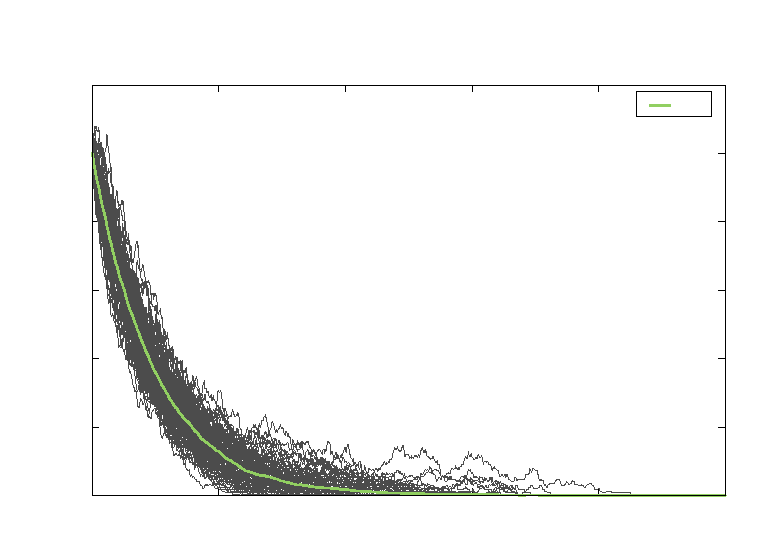
\includegraphics{graf12}}%
    \gplfronttext
  \end{picture}%
\endgroup
}
    \resizebox{0.49\linewidth}{!}{% GNUPLOT: LaTeX picture with Postscript
\begingroup
  \makeatletter
  \providecommand\color[2][]{%
    \GenericError{(gnuplot) \space\space\space\@spaces}{%
      Package color not loaded in conjunction with
      terminal option `colourtext'%
    }{See the gnuplot documentation for explanation.%
    }{Either use 'blacktext' in gnuplot or load the package
      color.sty in LaTeX.}%
    \renewcommand\color[2][]{}%
  }%
  \providecommand\includegraphics[2][]{%
    \GenericError{(gnuplot) \space\space\space\@spaces}{%
      Package graphicx or graphics not loaded%
    }{See the gnuplot documentation for explanation.%
    }{The gnuplot epslatex terminal needs graphicx.sty or graphics.sty.}%
    \renewcommand\includegraphics[2][]{}%
  }%
  \providecommand\rotatebox[2]{#2}%
  \@ifundefined{ifGPcolor}{%
    \newif\ifGPcolor
    \GPcolortrue
  }{}%
  \@ifundefined{ifGPblacktext}{%
    \newif\ifGPblacktext
    \GPblacktexttrue
  }{}%
  % define a \g@addto@macro without @ in the name:
  \let\gplgaddtomacro\g@addto@macro
  % define empty templates for all commands taking text:
  \gdef\gplbacktext{}%
  \gdef\gplfronttext{}%
  \makeatother
  \ifGPblacktext
    % no textcolor at all
    \def\colorrgb#1{}%
    \def\colorgray#1{}%
  \else
    % gray or color?
    \ifGPcolor
      \def\colorrgb#1{\color[rgb]{#1}}%
      \def\colorgray#1{\color[gray]{#1}}%
      \expandafter\def\csname LTw\endcsname{\color{white}}%
      \expandafter\def\csname LTb\endcsname{\color{black}}%
      \expandafter\def\csname LTa\endcsname{\color{black}}%
      \expandafter\def\csname LT0\endcsname{\color[rgb]{1,0,0}}%
      \expandafter\def\csname LT1\endcsname{\color[rgb]{0,1,0}}%
      \expandafter\def\csname LT2\endcsname{\color[rgb]{0,0,1}}%
      \expandafter\def\csname LT3\endcsname{\color[rgb]{1,0,1}}%
      \expandafter\def\csname LT4\endcsname{\color[rgb]{0,1,1}}%
      \expandafter\def\csname LT5\endcsname{\color[rgb]{1,1,0}}%
      \expandafter\def\csname LT6\endcsname{\color[rgb]{0,0,0}}%
      \expandafter\def\csname LT7\endcsname{\color[rgb]{1,0.3,0}}%
      \expandafter\def\csname LT8\endcsname{\color[rgb]{0.5,0.5,0.5}}%
    \else
      % gray
      \def\colorrgb#1{\color{black}}%
      \def\colorgray#1{\color[gray]{#1}}%
      \expandafter\def\csname LTw\endcsname{\color{white}}%
      \expandafter\def\csname LTb\endcsname{\color{black}}%
      \expandafter\def\csname LTa\endcsname{\color{black}}%
      \expandafter\def\csname LT0\endcsname{\color{black}}%
      \expandafter\def\csname LT1\endcsname{\color{black}}%
      \expandafter\def\csname LT2\endcsname{\color{black}}%
      \expandafter\def\csname LT3\endcsname{\color{black}}%
      \expandafter\def\csname LT4\endcsname{\color{black}}%
      \expandafter\def\csname LT5\endcsname{\color{black}}%
      \expandafter\def\csname LT6\endcsname{\color{black}}%
      \expandafter\def\csname LT7\endcsname{\color{black}}%
      \expandafter\def\csname LT8\endcsname{\color{black}}%
    \fi
  \fi
    \setlength{\unitlength}{0.0500bp}%
    \ifx\gptboxheight\undefined%
      \newlength{\gptboxheight}%
      \newlength{\gptboxwidth}%
      \newsavebox{\gptboxtext}%
    \fi%
    \setlength{\fboxrule}{0.5pt}%
    \setlength{\fboxsep}{1pt}%
\begin{picture}(7200.00,5040.00)%
    \gplgaddtomacro\gplbacktext{%
      \csname LTb\endcsname%%
      \put(1210,704){\makebox(0,0)[r]{\strut{}$-0.004$}}%
      \put(1210,1161){\makebox(0,0)[r]{\strut{}$-0.002$}}%
      \put(1210,1618){\makebox(0,0)[r]{\strut{}$0$}}%
      \put(1210,2076){\makebox(0,0)[r]{\strut{}$0.002$}}%
      \put(1210,2533){\makebox(0,0)[r]{\strut{}$0.004$}}%
      \put(1210,2990){\makebox(0,0)[r]{\strut{}$0.006$}}%
      \put(1210,3447){\makebox(0,0)[r]{\strut{}$0.008$}}%
      \put(1210,3905){\makebox(0,0)[r]{\strut{}$0.01$}}%
      \put(1210,4362){\makebox(0,0)[r]{\strut{}$0.012$}}%
      \put(1210,4819){\makebox(0,0)[r]{\strut{}$0.014$}}%
      \put(1342,484){\makebox(0,0){\strut{}$0$}}%
      \put(2409,484){\makebox(0,0){\strut{}$100$}}%
      \put(3475,484){\makebox(0,0){\strut{}$200$}}%
      \put(4542,484){\makebox(0,0){\strut{}$300$}}%
      \put(5608,484){\makebox(0,0){\strut{}$400$}}%
      \put(6675,484){\makebox(0,0){\strut{}$500$}}%
    }%
    \gplgaddtomacro\gplfronttext{%
      \csname LTb\endcsname%%
      \put(209,2761){\rotatebox{-270}{\makebox(0,0){\strut{}$u_1(t)$}}}%
      \put(4072,154){\makebox(0,0){\strut{}$t$}}%
      \csname LTb\endcsname%%
      \put(5879,3986){\makebox(0,0)[l]{\strut{}$m=100$}}%
      \csname LTb\endcsname%%
      \put(5879,4206){\makebox(0,0)[l]{\strut{}$m=50$}}%
      \csname LTb\endcsname%%
      \put(5879,4426){\makebox(0,0)[l]{\strut{}$m=25$}}%
      \csname LTb\endcsname%%
      \put(5879,4646){\makebox(0,0)[l]{\strut{}$m=16$}}%
    }%
    \gplbacktext
    \put(0,0){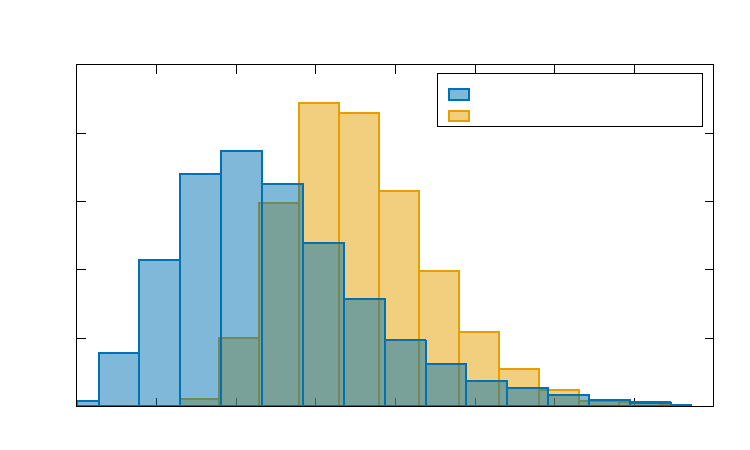
\includegraphics[width={360.00bp},height={252.00bp}]{graf13}}%
    \gplfronttext
  \end{picture}%
\endgroup
} \\
    \resizebox{0.49\linewidth}{!}{% GNUPLOT: LaTeX picture with Postscript
\begingroup
  \makeatletter
  \providecommand\color[2][]{%
    \GenericError{(gnuplot) \space\space\space\@spaces}{%
      Package color not loaded in conjunction with
      terminal option `colourtext'%
    }{See the gnuplot documentation for explanation.%
    }{Either use 'blacktext' in gnuplot or load the package
      color.sty in LaTeX.}%
    \renewcommand\color[2][]{}%
  }%
  \providecommand\includegraphics[2][]{%
    \GenericError{(gnuplot) \space\space\space\@spaces}{%
      Package graphicx or graphics not loaded%
    }{See the gnuplot documentation for explanation.%
    }{The gnuplot epslatex terminal needs graphicx.sty or graphics.sty.}%
    \renewcommand\includegraphics[2][]{}%
  }%
  \providecommand\rotatebox[2]{#2}%
  \@ifundefined{ifGPcolor}{%
    \newif\ifGPcolor
    \GPcolortrue
  }{}%
  \@ifundefined{ifGPblacktext}{%
    \newif\ifGPblacktext
    \GPblacktexttrue
  }{}%
  % define a \g@addto@macro without @ in the name:
  \let\gplgaddtomacro\g@addto@macro
  % define empty templates for all commands taking text:
  \gdef\gplbacktext{}%
  \gdef\gplfronttext{}%
  \makeatother
  \ifGPblacktext
    % no textcolor at all
    \def\colorrgb#1{}%
    \def\colorgray#1{}%
  \else
    % gray or color?
    \ifGPcolor
      \def\colorrgb#1{\color[rgb]{#1}}%
      \def\colorgray#1{\color[gray]{#1}}%
      \expandafter\def\csname LTw\endcsname{\color{white}}%
      \expandafter\def\csname LTb\endcsname{\color{black}}%
      \expandafter\def\csname LTa\endcsname{\color{black}}%
      \expandafter\def\csname LT0\endcsname{\color[rgb]{1,0,0}}%
      \expandafter\def\csname LT1\endcsname{\color[rgb]{0,1,0}}%
      \expandafter\def\csname LT2\endcsname{\color[rgb]{0,0,1}}%
      \expandafter\def\csname LT3\endcsname{\color[rgb]{1,0,1}}%
      \expandafter\def\csname LT4\endcsname{\color[rgb]{0,1,1}}%
      \expandafter\def\csname LT5\endcsname{\color[rgb]{1,1,0}}%
      \expandafter\def\csname LT6\endcsname{\color[rgb]{0,0,0}}%
      \expandafter\def\csname LT7\endcsname{\color[rgb]{1,0.3,0}}%
      \expandafter\def\csname LT8\endcsname{\color[rgb]{0.5,0.5,0.5}}%
    \else
      % gray
      \def\colorrgb#1{\color{black}}%
      \def\colorgray#1{\color[gray]{#1}}%
      \expandafter\def\csname LTw\endcsname{\color{white}}%
      \expandafter\def\csname LTb\endcsname{\color{black}}%
      \expandafter\def\csname LTa\endcsname{\color{black}}%
      \expandafter\def\csname LT0\endcsname{\color{black}}%
      \expandafter\def\csname LT1\endcsname{\color{black}}%
      \expandafter\def\csname LT2\endcsname{\color{black}}%
      \expandafter\def\csname LT3\endcsname{\color{black}}%
      \expandafter\def\csname LT4\endcsname{\color{black}}%
      \expandafter\def\csname LT5\endcsname{\color{black}}%
      \expandafter\def\csname LT6\endcsname{\color{black}}%
      \expandafter\def\csname LT7\endcsname{\color{black}}%
      \expandafter\def\csname LT8\endcsname{\color{black}}%
    \fi
  \fi
    \setlength{\unitlength}{0.0500bp}%
    \ifx\gptboxheight\undefined%
      \newlength{\gptboxheight}%
      \newlength{\gptboxwidth}%
      \newsavebox{\gptboxtext}%
    \fi%
    \setlength{\fboxrule}{0.5pt}%
    \setlength{\fboxsep}{1pt}%
\begin{picture}(7200.00,4320.00)%
    \gplgaddtomacro\gplbacktext{%
      \csname LTb\endcsname%%
      \put(616,408){\makebox(0,0)[r]{\strut{}$0$}}%
      \csname LTb\endcsname%%
      \put(616,1064){\makebox(0,0)[r]{\strut{}$0.05$}}%
      \csname LTb\endcsname%%
      \put(616,1720){\makebox(0,0)[r]{\strut{}$0.1$}}%
      \csname LTb\endcsname%%
      \put(616,2375){\makebox(0,0)[r]{\strut{}$0.15$}}%
      \csname LTb\endcsname%%
      \put(616,3031){\makebox(0,0)[r]{\strut{}$0.2$}}%
      \csname LTb\endcsname%%
      \put(616,3687){\makebox(0,0)[r]{\strut{}$0.25$}}%
      \csname LTb\endcsname%%
      \put(728,204){\makebox(0,0){\strut{}$2$}}%
      \csname LTb\endcsname%%
      \put(1492,204){\makebox(0,0){\strut{}$3$}}%
      \csname LTb\endcsname%%
      \put(2257,204){\makebox(0,0){\strut{}$4$}}%
      \csname LTb\endcsname%%
      \put(3021,204){\makebox(0,0){\strut{}$5$}}%
      \csname LTb\endcsname%%
      \put(3786,204){\makebox(0,0){\strut{}$6$}}%
      \csname LTb\endcsname%%
      \put(4550,204){\makebox(0,0){\strut{}$7$}}%
      \csname LTb\endcsname%%
      \put(5314,204){\makebox(0,0){\strut{}$8$}}%
      \csname LTb\endcsname%%
      \put(6079,204){\makebox(0,0){\strut{}$9$}}%
      \csname LTb\endcsname%%
      \put(6843,204){\makebox(0,0){\strut{}$10$}}%
    }%
    \gplgaddtomacro\gplfronttext{%
      \csname LTb\endcsname%%
      \put(4603,3198){\makebox(0,0)[l]{\strut{}$\beta =1$}}%
      \csname LTb\endcsname%%
      \put(4603,3402){\makebox(0,0)[l]{\strut{}$\beta_s =5 \beta, \, \beta_r=4\beta$}}%
      \csname LTb\endcsname%%
      \put(3785,3993){\makebox(0,0){\strut{}$N_0=250$}}%
    }%
    \gplbacktext
    \put(0,0){\includegraphics[width={360.00bp},height={216.00bp}]{graf14}}%
    \gplfronttext
  \end{picture}%
\endgroup
}
    \resizebox{0.49\linewidth}{!}{% GNUPLOT: LaTeX picture with Postscript
\begingroup
  \makeatletter
  \providecommand\color[2][]{%
    \GenericError{(gnuplot) \space\space\space\@spaces}{%
      Package color not loaded in conjunction with
      terminal option `colourtext'%
    }{See the gnuplot documentation for explanation.%
    }{Either use 'blacktext' in gnuplot or load the package
      color.sty in LaTeX.}%
    \renewcommand\color[2][]{}%
  }%
  \providecommand\includegraphics[2][]{%
    \GenericError{(gnuplot) \space\space\space\@spaces}{%
      Package graphicx or graphics not loaded%
    }{See the gnuplot documentation for explanation.%
    }{The gnuplot epslatex terminal needs graphicx.sty or graphics.sty.}%
    \renewcommand\includegraphics[2][]{}%
  }%
  \providecommand\rotatebox[2]{#2}%
  \@ifundefined{ifGPcolor}{%
    \newif\ifGPcolor
    \GPcolortrue
  }{}%
  \@ifundefined{ifGPblacktext}{%
    \newif\ifGPblacktext
    \GPblacktexttrue
  }{}%
  % define a \g@addto@macro without @ in the name:
  \let\gplgaddtomacro\g@addto@macro
  % define empty templates for all commands taking text:
  \gdef\gplbacktext{}%
  \gdef\gplfronttext{}%
  \makeatother
  \ifGPblacktext
    % no textcolor at all
    \def\colorrgb#1{}%
    \def\colorgray#1{}%
  \else
    % gray or color?
    \ifGPcolor
      \def\colorrgb#1{\color[rgb]{#1}}%
      \def\colorgray#1{\color[gray]{#1}}%
      \expandafter\def\csname LTw\endcsname{\color{white}}%
      \expandafter\def\csname LTb\endcsname{\color{black}}%
      \expandafter\def\csname LTa\endcsname{\color{black}}%
      \expandafter\def\csname LT0\endcsname{\color[rgb]{1,0,0}}%
      \expandafter\def\csname LT1\endcsname{\color[rgb]{0,1,0}}%
      \expandafter\def\csname LT2\endcsname{\color[rgb]{0,0,1}}%
      \expandafter\def\csname LT3\endcsname{\color[rgb]{1,0,1}}%
      \expandafter\def\csname LT4\endcsname{\color[rgb]{0,1,1}}%
      \expandafter\def\csname LT5\endcsname{\color[rgb]{1,1,0}}%
      \expandafter\def\csname LT6\endcsname{\color[rgb]{0,0,0}}%
      \expandafter\def\csname LT7\endcsname{\color[rgb]{1,0.3,0}}%
      \expandafter\def\csname LT8\endcsname{\color[rgb]{0.5,0.5,0.5}}%
    \else
      % gray
      \def\colorrgb#1{\color{black}}%
      \def\colorgray#1{\color[gray]{#1}}%
      \expandafter\def\csname LTw\endcsname{\color{white}}%
      \expandafter\def\csname LTb\endcsname{\color{black}}%
      \expandafter\def\csname LTa\endcsname{\color{black}}%
      \expandafter\def\csname LT0\endcsname{\color{black}}%
      \expandafter\def\csname LT1\endcsname{\color{black}}%
      \expandafter\def\csname LT2\endcsname{\color{black}}%
      \expandafter\def\csname LT3\endcsname{\color{black}}%
      \expandafter\def\csname LT4\endcsname{\color{black}}%
      \expandafter\def\csname LT5\endcsname{\color{black}}%
      \expandafter\def\csname LT6\endcsname{\color{black}}%
      \expandafter\def\csname LT7\endcsname{\color{black}}%
      \expandafter\def\csname LT8\endcsname{\color{black}}%
    \fi
  \fi
    \setlength{\unitlength}{0.0500bp}%
    \ifx\gptboxheight\undefined%
      \newlength{\gptboxheight}%
      \newlength{\gptboxwidth}%
      \newsavebox{\gptboxtext}%
    \fi%
    \setlength{\fboxrule}{0.5pt}%
    \setlength{\fboxsep}{1pt}%
\begin{picture}(11338.00,10204.00)%
    \gplgaddtomacro\gplbacktext{%
    }%
    \gplgaddtomacro\gplfronttext{%
      \csname LTb\endcsname%%
      \put(5635,9873){\makebox(0,0){\Huge $T=2.5$}}%
    }%
    \gplbacktext
    \put(0,0){\includegraphics{graf15}}%
    \gplfronttext
  \end{picture}%
\endgroup
}
    \caption{Vstopni signali dobljeni z~rezanjem filtriranega območja -- $m$ je njihova 
    širina.}
    \label{slika9}
\end{figure}

%----------------------------------------------------------------------------------------
%	PROBLEM 3
%----------------------------------------------------------------------------------------
\section{Čiščenje slike}
V~arhivu \path{lena_slike.tar.gz} imamo slike podobe Lene, ki so razmazane s~tremi znanimi
konvolucijskimi jedri: tresoč objektiv (\path{kernel1.pgm}, slab fokus (\path{kernel2.pgm}
ter uklonska mrežica (\path{kernel3.pgm}). Datotekam je primešana različna količina
Gaussovega šuma (RMS $= 0,4,8,16$). Po filtriranju z~uporabo Wienerjevega filtra 
rekonstruiramo slike. V~arhivu so tudi slike z~dodano periodično motnjo (\path{*_nx.pgm}).
\subsection{Pristop}
Problema se lotimo na enak način kot v~prejšnjem odseku, le da tukaj Wienerjev filter
prepišemo v~drugo obliko:
\begin{equation}
    \Phi (\omega) = \frac{1}{R(\omega)} \frac{|R(\omega)|^2}{|R(\omega)|^2 + 
    \frac{N(\omega)}{S(\omega)}}
\end{equation}
Sliko po stolpcih preberemo in vsak posamezen stolpec, na enak način kot v~prejšnjem delu, 
rekonstruiramo. Zopet upoštevamo nek \emph{cut off} šuma in poskusimo očistiti sliko.
Slike brez dodanega gaussovega šuma lahko kar rekonstruiramo brez uporabe Wienerjevega 
filtra.
\subsection{Dobljene slike}
Najprej si poglejmo slike brez dodanega Gaussovega šuma:
\begin{figure}[H]
    \centering
    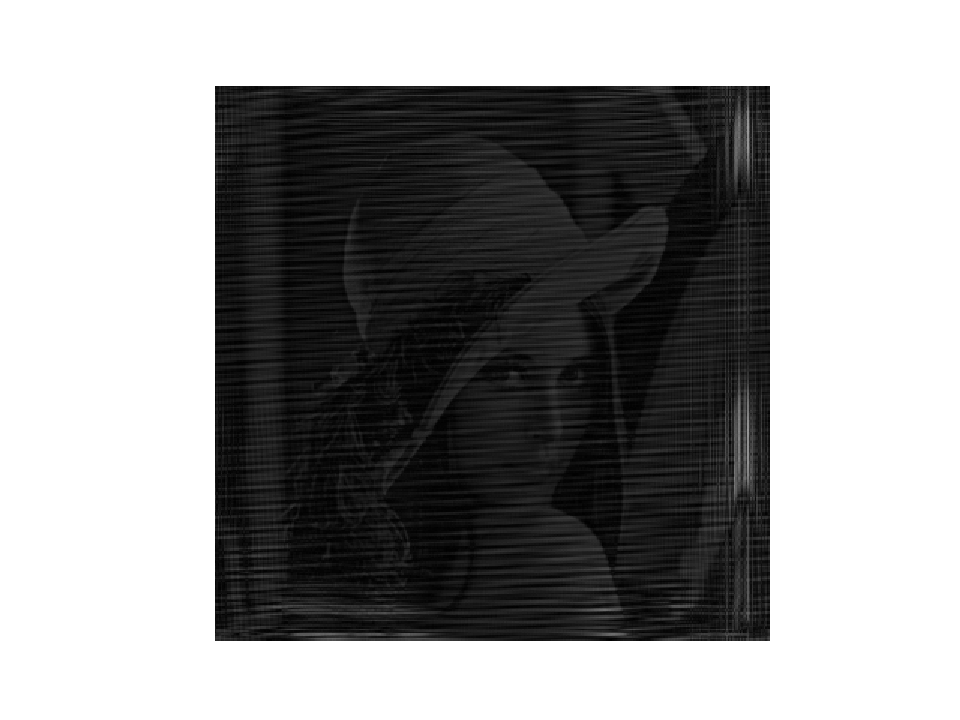
\includegraphics[width=0.3\textwidth]{3naloga/ociscena_lena_k1_n0.pdf}
    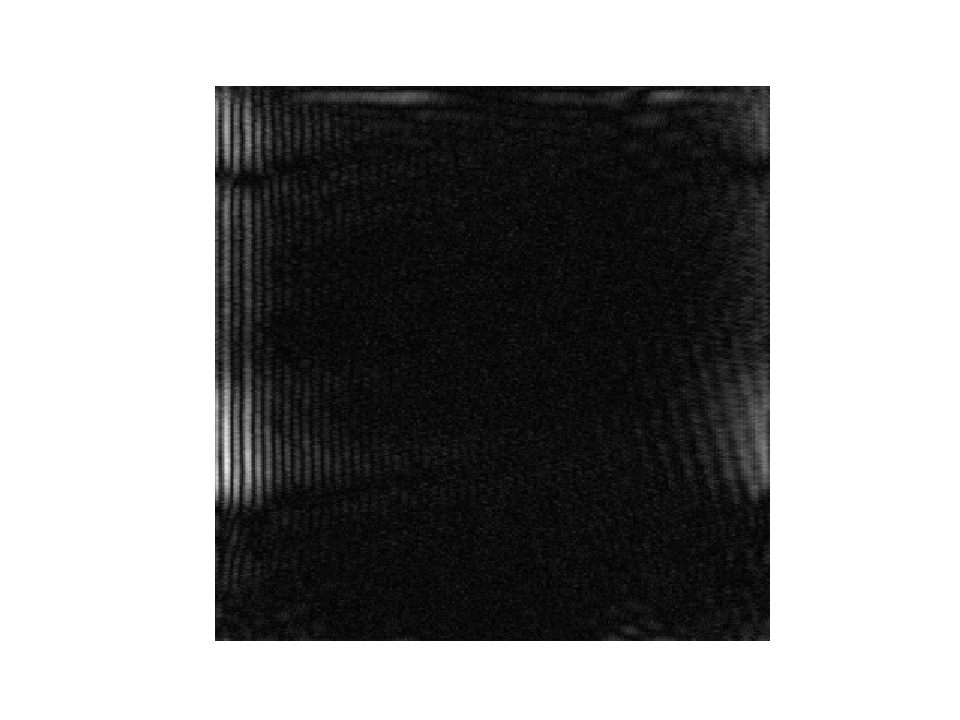
\includegraphics[width=0.3\textwidth]{3naloga/ociscena_lena_k2_n0.pdf}
    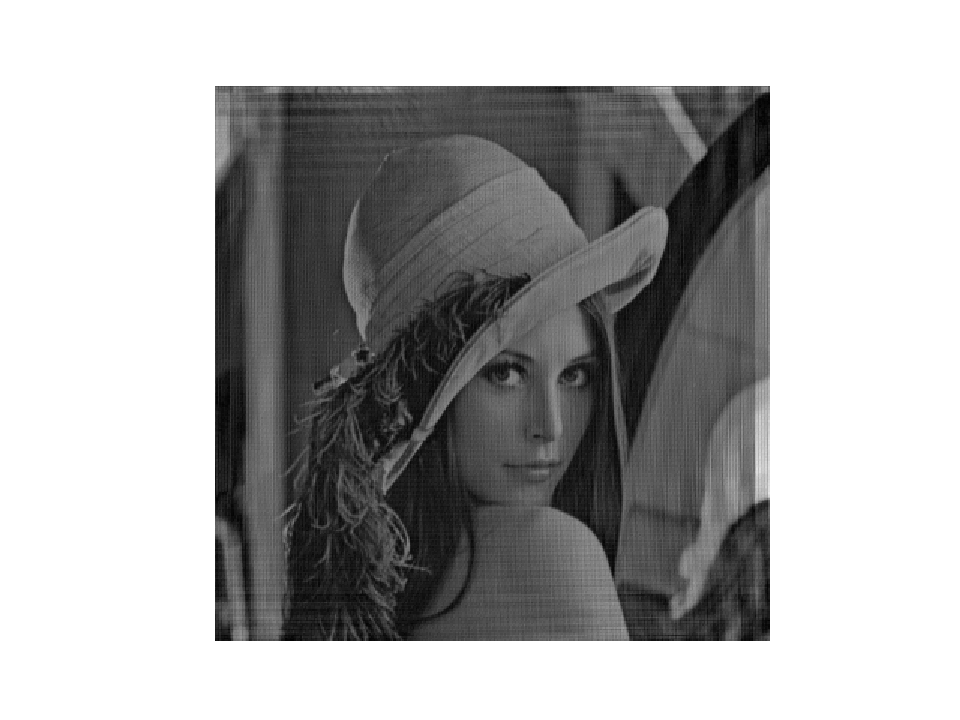
\includegraphics[width=0.3textwidth]{3naloga/ociscena_lena_k3_n0.pdf}
    \caption{Očiščene slike brez dodanega šuma -- od leve proti desni: 
    \protect\path{k1-n0}, \protect\path{k2-n0} in \protect\path{k3-n0}.}
    \label{slika10}
\end{figure}
vidimo, da je najlepše očiščena tretja slika, druga slika precej neprepoznavna, prva je 
sicer zatemnjena, vendar razločimo sliko. Poglejmo si najprej očiščene vse slike s~tretjim
jedrom.

\begin{figure}[H]
    \centering
    \includegraphics[width=0.25\textwidth]{temp/ociscena-k3-n4.pdf}
    \includegraphics[width=0.25\textwidth]{temp/ociscena-k3-n8.pdf}\\
    \includegraphics[width=0.25\textwidth]{temp/ociscena-k3-n16.pdf}
    \includegraphics[width=0.25\textwidth]{temp/ociscena-k3-nx.pdf}
    \caption{Očiščene slike s~tretjim jedrom -- v~zgosnji vrsti: \protect\path{k3-n4}, 
    \protect\path{k3-n8} in v~spodnji: \protect\path{k3-n16} ter \protect\path{k3-nx}.}
    \label{slika11}
\end{figure}
Poskusimo očistiti tudi slike s~prvim jedrom, vendar že za najmanjši šum pride rešitev
precej zatemnjena in nerazpoznavna.
\begin{figure}[H]
    \centering
    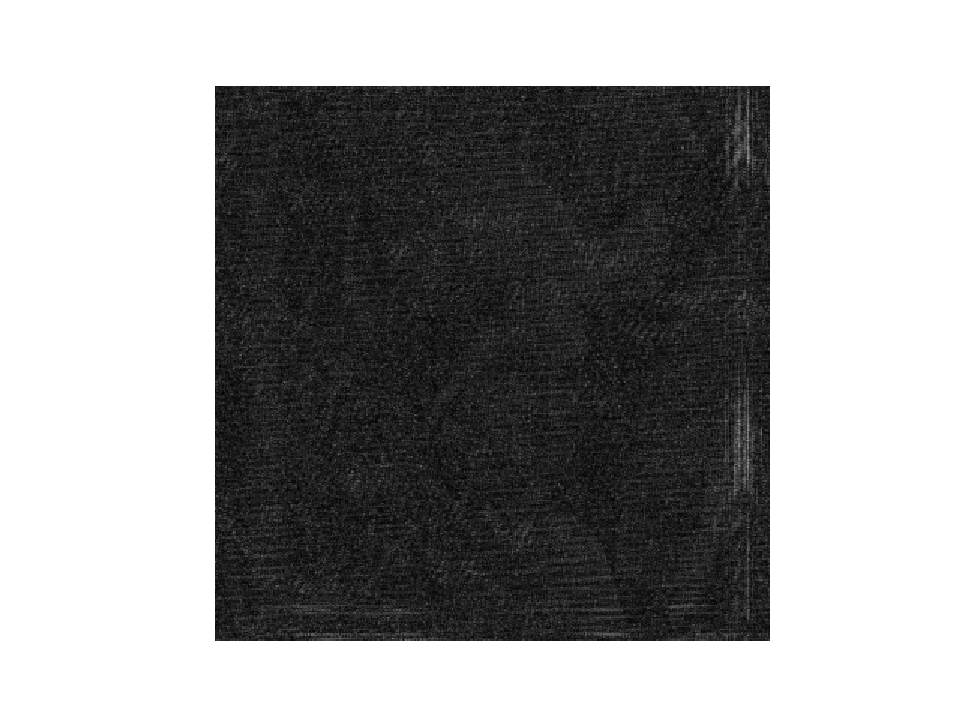
\includegraphics[width=0.5\textwidth]{temp/ociscena-k1-n4.pdf}
    \caption{Poskus čiščenja slike: \protect\path{k1-n4}}
    \label{slika12}
\end{figure}
Druge slike ne uspemo očistiti, poskusimo z~različnimi variacijami filtra in širinami 
frekvenčnih območij, ki jih odrežemo, morda bi morali poskusiti s~kakšnim drugačnim jedrom.
\end{document}
